\documentclass[9pt]{article}
\usepackage[top=3cm,bottom=4cm,inner=2cm,outer=2cm]{geometry}

\usepackage{amsmath}
\usepackage{siunitx}
\usepackage{graphicx}
\usepackage{booktabs}
\usepackage{hyperref}
\usepackage{float}
\usepackage{hyperref}

\title{Pound-Drever-Hall Locking: A Frequency-Domain Model}
\author{PDH learning project --- \textit{source/PDH}}
\date{\today}

\begin{document}
\maketitle

\begin{abstract}
This is a slow, worked-example companion to the MATLAB model built under
\textit{source/PDH}, whose purpose is to \emph{learn} Pound-Drever-Hall (PDH)
laser frequency stabilization by reproducing the physics of the Liquid
Instruments webinar ``High-Performance PDH Locking with Reconfigurable
Instrumentation'' (J.\ Miller, 2024) section by section, in code, and
cross-checking every derivation numerically rather than trusting it by
inspection. Section~\ref{sec:cavity} covers the passive Fabry-P\'erot cavity:
where its three characteristic numbers (FSR, Finesse, linewidth) come from,
and where the reflection/transmission formulas themselves come from, derived
as a geometric series over round trips. Section~\ref{sec:sidebands} covers
phase modulation: why PDH needs sidebands at all, the Jacobi-Anger expansion
that produces them, and the phasor picture that makes the counter-rotating
sidebands visualizable. Section~\ref{sec:pdh-detection} builds the explicit
photodiode/mixer/low-pass-filter detection chain that turns the reflected
field into the PDH error signal. Section~\ref{sec:pdh-dotproduct} reframes
that same error signal as a single geometric dot product between the
carrier's own reflected phasor and the sideband resultant, worked through at
four characteristic detunings. This completes the frequency-domain model the
underlying wayfinder map (\textit{.scratch/pdh-frequency-domain-model/}) set
out to build; the closed-loop time-domain servo simulation (PI controller,
simulated PZT actuator, lock acquisition) is a separate, later effort.
\end{abstract}

\section{The Fabry-P\'erot Cavity}
\label{sec:cavity}
\subsection{The physical picture}
\label{sec:cavity-picture}
A Fabry-P\'erot cavity is two mirrors facing each other, separated by a
length. Send a laser in through one mirror. The light bounces back and
forth: a little bit leaks out through each mirror on every pass, and what
leaks out interferes with what leaked out on previous passes. Whether that
interference is constructive or destructive depends entirely on how many
wavelengths fit exactly into one round trip --- which depends on the laser's
frequency. That is the entire mechanism: frequency selects resonance because
frequency sets the round-trip phase.

Everything about the cavity's response reduces to three quantities, computed
by the \textit{OpticalCavity} class from four physical inputs: the cavity
length, the laser wavelength, and the two mirrors' power reflectivities. The
reflection and transmission formulas derived below follow
\cite{black2001pdh}, Eqs.~5--6. Table~\ref{tab:cavity-glossary} collects the
notation.
\begin{table}[H]
\centering
\small
\begin{tabular}{@{}llp{6.8cm}@{}}
\toprule
Symbol & Code identifier & Meaning \\
\midrule
$L$ & \textit{CavityLength} & mirror separation (round-trip length), \si{\meter} \\
$\lambda$ & \textit{Wavelength} & laser vacuum wavelength, \si{\meter} \\
$n(\lambda)$ & \textit{RefractiveIndex} & medium refractive index; scalar or dispersive function handle \\
$R_1, R_2$ & \textit{InputMirrorPowerReflectivity}, \textit{BackMirrorPowerReflectivity} & mirror power reflectivities \\
$r_1, r_2$ & (private) \textit{mirrorAmplitudeReflectivities} & amplitude reflectivities, $r_i = \sqrt{R_i}$ \\
$t_1, t_2$ & --- & amplitude transmissivities, $t_i = \sqrt{1-R_i}$ (lossless mirror) \\
$g$ & --- & round-trip amplitude reflectivity, $g = r_1 r_2$ \\
$\mathrm{FSR}$ & \textit{get.FSR} & free spectral range, \si{\hertz} (Eq.~\eqref{eq:fsr}) \\
$N$ & --- & integer resonance mode number (Eq.~\eqref{eq:mode-comb}); \emph{not} the round-trip index $k$ of Eqs.~\eqref{eq:transmission}--\eqref{eq:reflection} \\
$f_{\mathrm{laser}}$ & --- & the laser's actual frequency (Eq.~\eqref{eq:detuning-def}) \\
$f_{0,N}$ & --- & the $N$-th resonance's frequency (Eq.~\eqref{eq:mode-comb}) \\
$\Delta f_{\mathrm{detune}}$ & argument \textit{detuningHz} & laser detuning from the nearest cavity resonance, \si{\hertz} (Eq.~\eqref{eq:detuning-def}) \\
$\varphi$ & \textit{roundTripPhase} & round-trip phase accumulated at detuning $\Delta f_{\mathrm{detune}}$ \\
$\mathcal{F}$ & \textit{get.Finesse} & cavity finesse (Eq.~\eqref{eq:finesse}) \\
$\Delta\nu_{\mathrm{FWHM}}$ & \textit{get.LinewidthFWHM} & resonance linewidth, FWHM, \si{\hertz} (Eq.~\eqref{eq:linewidth}) \\
$r(\varphi)$ & \textit{reflectionCoefficient} & the cavity's overall complex reflection coefficient (Eq.~\eqref{eq:reflection}) --- not to be confused with the per-mirror $r_1,r_2$ above \\
$T_1, T_2$ & --- & mirror power transmissivities, $T_i=1-R_i$ (\S\ref{sec:cavity-coupling}) \\
\bottomrule
\end{tabular}
\caption{Notation used throughout Section~\ref{sec:cavity}.}
\label{tab:cavity-glossary}
\end{table}
\subsection{The three numbers: FSR, Finesse, linewidth}
\label{sec:cavity-three-numbers}
\textbf{Free Spectral Range (FSR).} The frequency spacing between one
resonance and the next. The round-trip time is $2n(\lambda)L/c$ (there and
back, through a medium of index $n(\lambda)$), so the light returns ``in phase'' only
at frequencies spaced by the round-trip rate:
\begin{equation}
\mathrm{FSR} = \frac{c}{2\, n(\lambda)\, L}.
\label{eq:fsr}
\end{equation}
For the running example used throughout this report --- $L=\SI{14.9896229}{\centi\meter}$,
$\lambda = \SI{1064}{\nano\meter}$, vacuum ($n=1$) --- this evaluates to exactly $\mathrm{FSR}=\SI{1}{\giga\hertz}$.
% CHECKED-BY: ReportClaimsCavityTest.fsrIsExactlyOneGigahertz

The cavity's resonances form a discrete comb of longitudinal modes, indexed
by an integer mode number $N$, with resonance frequencies
\begin{equation}
f_{0,N} = f_{0,0} + N \cdot \mathrm{FSR},
\label{eq:mode-comb}
\end{equation}
spaced by exactly one FSR apart. The laser's detuning from whichever mode it
currently sits nearest is
\begin{equation}
\Delta f_{\mathrm{detune}} = f_{\mathrm{laser}} - f_{0,N},
\label{eq:detuning-def}
\end{equation}
the same quantity passed as \textit{detuningHz} throughout \textit{OpticalCavity}
(Table~\ref{tab:cavity-glossary}).

\textbf{Finesse.} How sharp each resonance is, in units of ``how many
resonances would fit across one linewidth.'' Better mirrors (higher
reflectivity) keep light bouncing longer, so a resonance can be a narrower
sliver of frequency before it stops building up:
\begin{equation}
\mathcal{F} = \frac{\pi\sqrt{g}}{1-g}, \qquad g = r_1 r_2.
\label{eq:finesse}
\end{equation}
This is \textit{get.Finesse}, line-for-line.

\textbf{Linewidth (FWHM).} The actual width, in \si{\hertz}, of a resonance
dip or peak:
\begin{equation}
\Delta\nu_{\mathrm{FWHM}} = \frac{\mathrm{FSR}}{\mathcal{F}}.
\label{eq:linewidth}
\end{equation}
This is \textit{get.LinewidthFWHM} --- almost a tautology once
Eqs.~\eqref{eq:fsr}--\eqref{eq:finesse} exist, since Finesse is \emph{defined}
as that ratio.

Table~\ref{tab:finesse-vs-reflectivity} makes the Finesse$\leftrightarrow$reflectivity$\leftrightarrow$linewidth
relationship concrete: FSR is held fixed at \SI{1}{\giga\hertz} while the
(matched) mirror reflectivity improves. Each $10\times$ improvement in mirror
quality ($1-R$ shrinking by $10\times$) gives roughly $10\times$ the Finesse
and $10\times$ narrower linewidth. The last column,
$\pi/(1-R)$, is the textbook high-reflectivity approximation to
Eq.~\eqref{eq:finesse}; it only approaches the exact value as $R\to1$, since
it drops the $\sqrt{g}\to1$ approximation's own residual error.
\begin{table}[H]
\centering
\begin{tabular}{@{}llll@{}}
\toprule
$R = R_1 = R_2$ & Finesse & Linewidth (FWHM) & $\pi/(1-R)$ \\
\midrule
0.9000 & 29.8 & \SI{3.355e+07}{\hertz} & 31.4 \\
0.9900 & 312.6 & \SI{3.199e+06}{\hertz} & 314.2 \\
0.9990 & 3140.0 & \SI{3.185e+05}{\hertz} & 3141.6 \\
0.9999 & 31414.4 & \SI{3.183e+04}{\hertz} & 31415.9 \\
\bottomrule
\end{tabular}

\caption{Finesse and linewidth vs. matched mirror power reflectivity $R$, at
fixed $\mathrm{FSR}=\SI{1}{\giga\hertz}$. Generated by
\textit{generateReportFigures.m} (\textit{exportFinesseTable}) directly from
\textit{OpticalCavity}, so it can never silently drift from the code.}
\label{tab:finesse-vs-reflectivity}
\end{table}
\subsection{Deriving the reflection and transmission coefficients}
\label{sec:cavity-derivation}
This is the part worth understanding, not just trusting. Inside the cavity,
light does not bounce just once --- it bounces over and over, and every one
of those escaping ``echoes'' adds up coherently. Each round trip multiplies
the intracavity field by $g\,e^{i\varphi}$ (mirror reflectivities times the
phase $\varphi = 2\pi\Delta f_{\mathrm{detune}}/\mathrm{FSR}$ picked up traversing the round-trip
length at detuning $\Delta f_{\mathrm{detune}}$). So the transmitted field is a geometric series
over round-trip number $k$ (deliberately not $N$, reserved above for the
resonance mode number, Eq.~\eqref{eq:mode-comb}):
\begin{equation}
\frac{E_{\mathrm{trans}}}{E_{\mathrm{in}}}
= t_1 t_2 \sum_{k=0}^{\infty} \left(g\,e^{i\varphi}\right)^k
= \frac{t_1 t_2}{1 - g\,e^{i\varphi}}.
\label{eq:transmission}
\end{equation}
This is exactly \textit{transmissionCoefficient}'s formula. Figure~\ref{fig:convergence}
does not take this on faith: it sums the series numerically to a finite
number of round trips and plots the residual error against the exact closed
form, on resonance, for two different finesse values. The convergence rate is
set by how quickly $g^k$ decays --- controlled by the same $1-g$ that sets the
Finesse in Eq.~\eqref{eq:finesse}. High finesse literally means ``light
survives many round trips before it decays,'' and that is why the resonance
is narrow: a signal that persists longer in time is confined to a narrower
band in frequency, the same time$\leftrightarrow$frequency tradeoff behind
every resonance.
\begin{figure}[H]
\centering
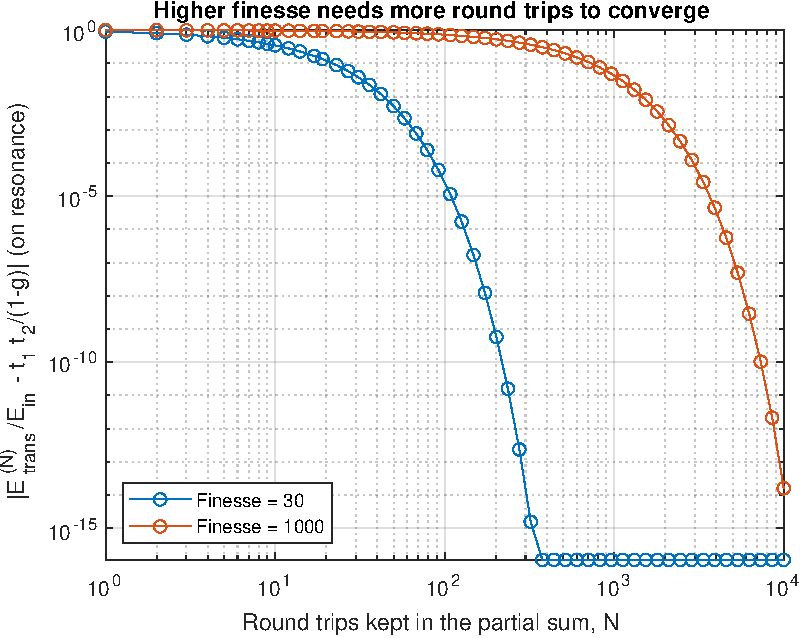
\includegraphics[width=0.8\textwidth]{pic/geometric-series-convergence.pdf}
\caption{Convergence of the truncated geometric series
(Eq.~\eqref{eq:transmission}, first $k$ terms) to the exact closed form, on
resonance, for a low-finesse and a high-finesse cavity. The high-finesse
cavity needs roughly $100\times$ more round trips to reach the same
residual error --- the numerical face of ``narrower linewidth needs more
round trips to build up.''}
\label{fig:convergence}
\end{figure}
\textbf{Reflection: one extra term, same idea.} The transmitted field above
is only the leaked-out geometric series. The reflected field has that too,
but it also gets the light that bounces straight off the front mirror
without ever entering the cavity:
\begin{equation}
\frac{E_{\mathrm{refl}}}{E_{\mathrm{in}}}
= -r_1 + t_1^2\, r_2\, e^{i\varphi} \sum_{k=0}^{\infty}\left(g\,e^{i\varphi}\right)^k
= \frac{r_2\, e^{i\varphi} - r_1}{1 - g\, e^{i\varphi}}
\label{eq:reflection}
\end{equation}
after substituting $t_1^2 = 1-r_1^2$ and simplifying. This is exactly
\textit{reflectionCoefficient}'s formula. For a symmetric cavity
($r_1=r_2=r$), setting $\varphi=0$ gives $(r-r)/(1-r^2)=0$: the direct
reflection off the front mirror exactly cancels the light leaking back out,
on resonance. All the power that came in has to go somewhere, and with
nothing reflected, it all goes through --- exactly the ``reflection dips to
0, transmission peaks to 1'' picture in Figure~\ref{fig:cavity-response}
below. Note the structural difference from Eq.~\eqref{eq:transmission}: the
reflection formula has a $-r_1$ term sitting outside the round-trip sum;
transmission is only the leaked-out buildup, reflection is that buildup
\emph{minus} the direct bounce.

\subsection{Reading the cavity response}
\label{sec:cavity-response}
\begin{figure}[H]
\centering
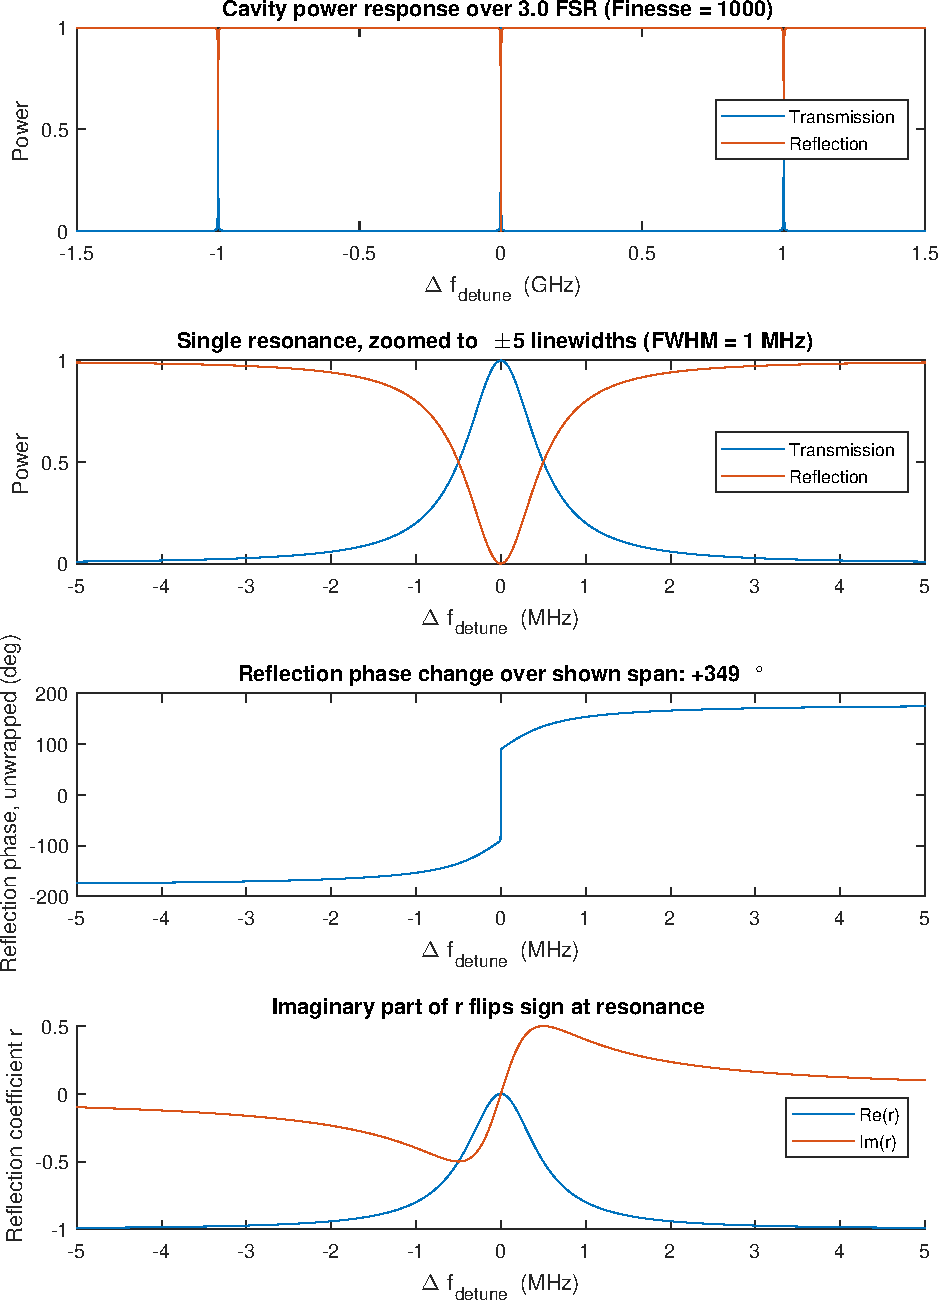
\includegraphics[width=0.75\textwidth]{pic/cavity-response.pdf}
\caption{The running-example cavity's response ($\mathrm{FSR}=\SI{1}{\giga\hertz}$,
$\mathcal{F}=1000$), produced by \textit{plotCavityResponse.m}.}
\label{fig:cavity-response}
\end{figure}
Reading each panel of Figure~\ref{fig:cavity-response} with the physics of
Sections~\ref{sec:cavity-three-numbers}--\ref{sec:cavity-derivation} in hand:

\begin{itemize}
\item \textbf{Panel 1} (wide scan, $\pm1.5\,\mathrm{FSR}$): three narrow
spikes, one full \si{\giga\hertz} apart --- that spacing is the FSR of
Eq.~\eqref{eq:fsr}. At this zoom the resonances look like infinitely thin
lines because the linewidth (\SI{1}{\mega\hertz}) is a thousandth of the FSR
(\SI{1}{\giga\hertz}) --- a direct visual of ``Finesse $=1000$'': a thousand
resonance-widths would fit between one resonance and the next.
\item \textbf{Panel 2} (zoomed to $\pm5$ linewidths): the geometric series
made visible. Transmission peaks exactly at 1 on resonance --- light built up
over thousands of round trips, all constructively interfering, escaping
fully. One linewidth away, the round-trip phase $\varphi$ has drifted enough
that after many round trips the interference is no longer constructive:
transmission collapses, reflection recovers. The width of that collapse is
the linewidth of Eq.~\eqref{eq:linewidth}.
\item \textbf{Panel 3} (reflection phase): the panel that matters most for
PDH. Off resonance, the reflected light is basically just the direct bounce
off the front mirror --- nothing subtle. But near resonance, the reflected
field's \emph{amplitude} passes through zero (Panel 2's red curve), and
amplitude passing through zero is a phase singularity: the phasor has to
spin around to get from ``pointing one way'' to ``pointing the opposite
way'' as detuning crosses zero. That spin is the steep $360^\circ$ jump seen
here. This phase response is the entire reason PDH works: it is a fast,
sign-changing signal that can be extracted electronically and fed back to
keep a laser locked to resonance --- but a photodiode only measures power,
not phase, which is exactly why Section~\ref{sec:sidebands} exists.
\item \textbf{Panel 4} (real/imaginary parts of the reflection coefficient):
the same phase information as Panel 3, decomposed into Cartesian components.
$\mathrm{Im}(r)$ is the antisymmetric, dispersive-shaped curve that flips
sign exactly at resonance --- this is the curve PDH's error signal is built
to reproduce electronically (Section~\ref{sec:sidebands} and later
sections), and its shape is the direct payoff of Eq.~\eqref{eq:reflection}
passing through zero.
\end{itemize}

\subsection{A worked conceptual check: what destructively interferes with what}
\label{sec:cavity-conceptual-check}
It is tempting to describe on-resonance cancellation as ``all the round
trips destructively interfere with each other.'' That is not quite right,
and the distinction matters for what follows.

Recall detuning $\Delta f_{\mathrm{detune}}$ (Eq.~\eqref{eq:detuning-def}),
measured from whichever resonance mode (Eq.~\eqref{eq:mode-comb}) the laser
currently sits nearest to --- the three peaks in
Figure~\ref{fig:cavity-response}'s Panel~1 are three such modes. It is what
labels every panel of Figure~\ref{fig:phasor-chain-conceptual} below.
\begin{figure}[H]
\centering
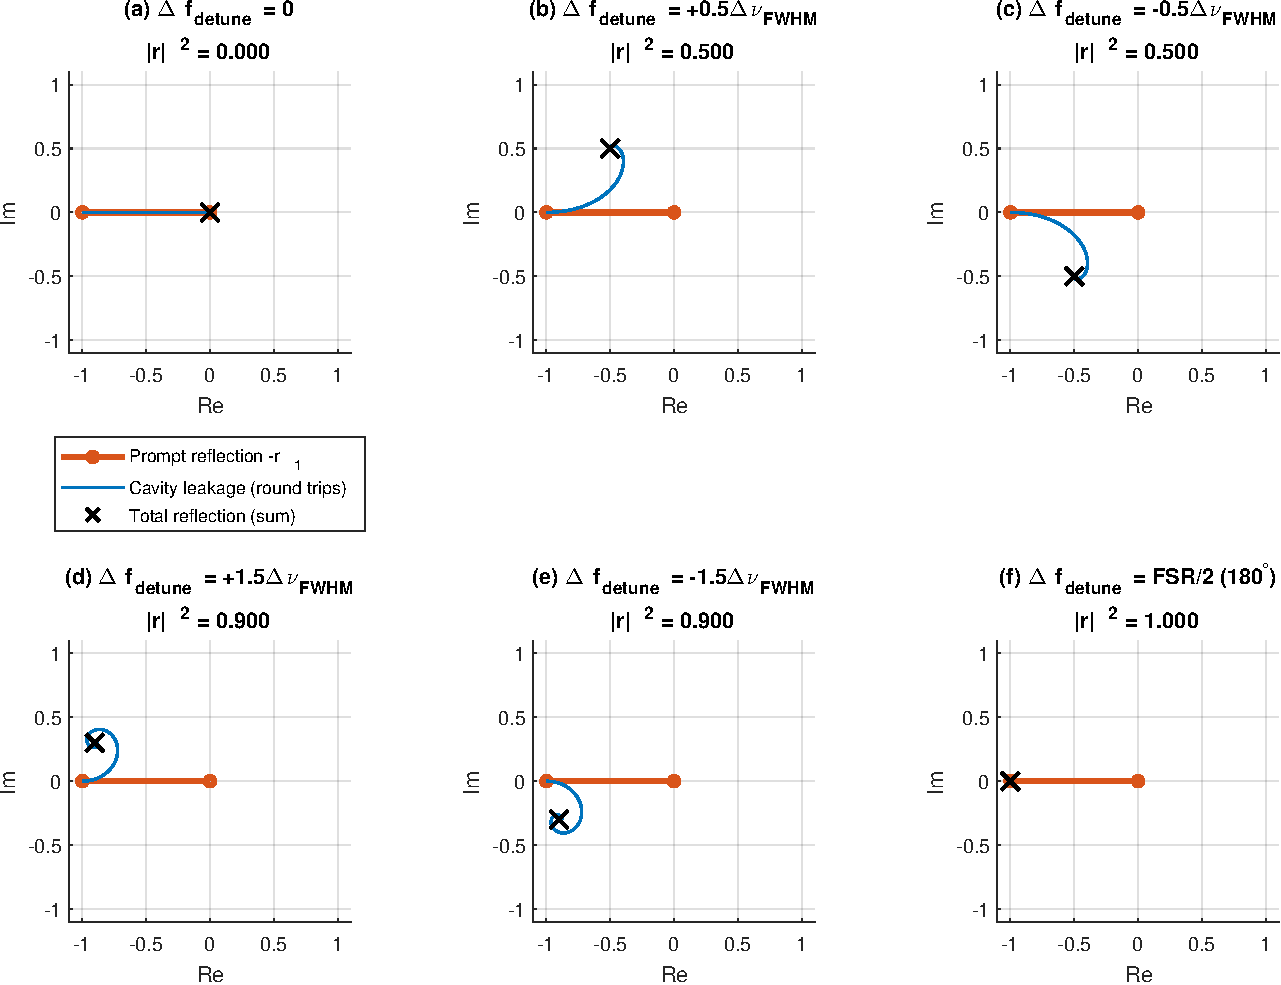
\includegraphics[width=\textwidth]{pic/phasor-chain-conceptual.pdf}
\caption{The round-trip phasor chain of Eq.~\eqref{eq:reflection}, drawn
head-to-tail, for this report's running-example cavity ($\mathrm{FSR}=\SI{1}{\giga\hertz}$,
$\mathcal{F}=1000$, the same cavity as Figure~\ref{fig:cavity-response}), at
six fixed values of $\Delta f_{\mathrm{detune}}$ (Eq.~\eqref{eq:detuning-def}).
Orange: the prompt reflection $-r_1$, the direct bounce off the front
mirror, with filled endpoints at the origin and at $-r_1$. Blue: the
cavity's leaked-out buildup, the geometric series of
Eq.~\eqref{eq:transmission}-like round-trip echoes --- drawn as a smooth
curve rather than a hand-countable chain of arrows, since at this finesse
thousands of round trips are needed to converge (recall the Finesse$=1000$
curve of Figure~\ref{fig:convergence}). Black \texttt{x}: the exact
closed-form total, Eq.~\eqref{eq:reflection}, confirming the sum lands in
the right place. Panel (a) is on resonance ($\Delta f_{\mathrm{detune}}=0$);
(b)/(c) are $\pm0.5$ and (d)/(e) are $\pm1.5$ of this cavity's own linewidth
(Eq.~\eqref{eq:linewidth}) away from it; (f) is $\Delta
f_{\mathrm{detune}}=\mathrm{FSR}/2$, the $180^\circ$ anti-resonance point
(maximum reflection, always exactly half an FSR away regardless of
finesse). Detunings are expressed as fractions of the linewidth rather than
fixed absolute degrees, since at $\mathcal{F}=1000$ the resonance itself is
only $360^\circ/1000=0.36^\circ$ of round-trip phase wide --- fixed angles
like $\pm30^\circ$ or $\pm90^\circ$ would all land far outside it and look
identical (reflected power $>0.9999$ in every case). As $\Delta
f_{\mathrm{detune}}$ is swept continuously rather than sampled at six fixed
points, the black \texttt{x} traces out a full circle in the complex plane
--- the \emph{resonance circle} formalized in
Section~\ref{sec:cavity-coupling} (Figure~\ref{fig:coupling-regimes}).}
\label{fig:phasor-chain-conceptual}
\end{figure}
Figure~\ref{fig:phasor-chain-conceptual} makes the two-term structure of
Eq.~\eqref{eq:reflection} literal. In every panel, the blue leakage curve
itself always builds \emph{outward} from $-r_1$ --- the individual round
trips are interfering \emph{constructively} with each other, building up
coherently; if they destructively cancelled among themselves instead,
nothing would build up and there would be no resonance to speak of. What
changes from panel to panel is only where that curve's final tip lands
relative to the orange prompt-reflection arrow. In panel (a) (on resonance),
the curve's tip lands exactly opposite the tip of the orange arrow, as seen
from the origin: added together, they cancel completely, $|r|^2=0$. That is
a one-on-one cancellation between two vectors, not a many-way cancellation
among the blue curve's own contributions. Moving off resonance (panels
(b)/(c), half a linewidth either side), the curve's final tip rotates away
from that exactly-opposite point, so the two vectors no longer fully cancel
and $|r|^2$ rises to $0.5$ --- symmetric in sign, since $\pm0.5$ linewidths
give the same $|r|^2$.
% CHECKED-BY: ReportClaimsCavityTest.reflectedPowerRisesToOneHalfAtHalfLinewidth
Panels (d)/(e) ($\pm1.5$ linewidths) show the curve
rotated further still, well past the point of cancellation, $|r|^2=0.9$.
% CHECKED-BY: ReportClaimsCavityTest.reflectedPowerIsZeroPointNineAtOnePointFiveLinewidths
Panel (f) ($180^\circ$, anti-resonance) shows the curve's tip swinging
around to point in the \emph{same} direction as the orange arrow --- here
the two vectors add rather than cancel, giving this cavity's maximum
reflection, $|r|^2\approx1$ (Section~\ref{sec:cavity-three-numbers}'s power
conservation applies at every detuning, not only on resonance --- at this
much higher finesse than the earlier numeric example, almost none of the
power is transmitted at the point of maximum reflection).

Detuning does not ``destroy the reflection''; it destroys the
\emph{cancellation}, letting reflection recover back up toward~1 (numerically:
at a fixed \SI{1}{\mega\hertz} detuning, reflected power goes from $0.0035$
at $\mathcal{F}=30$ to $0.9997$ at $\mathcal{F}\approx31000$
% CHECKED-BY: ReportClaimsCavityTest.reflectedPowerAtFixedDetuningGrowsWithFinesse
--- a higher-finesse
cavity has a narrower resonance, so the same fixed detuning sits further
outside it, and the interference there looks less and less destructive). At
exact resonance, reflection is already at its minimum; detuning is what
undoes the destructive interference and gives the reflected light back.

\subsection{Over- and undercoupled cavities}
\label{sec:cavity-coupling}
Every cavity used so far has had matched mirrors, $R_1=R_2$. That is a
special case, called \emph{critical coupling}, and real cavities do not have
to satisfy it. Whether a cavity is under-, critically, or over-coupled
compares two rates: how fast power couples in and back out through the front
mirror, set by $T_1=1-R_1$, against how fast power escapes by every other
route --- in this lossless two-mirror model, that means solely through the
back mirror, set by $T_2=1-R_2$. In terms of the mirror reflectivities
already in use throughout this report:
\begin{itemize}
\item \textbf{Critically coupled} ($R_1=R_2$): the two rates match. Setting
$\varphi=0$ in Eq.~\eqref{eq:reflection} gives $r(0)=0$ exactly --- every
watt that enters the cavity eventually leaves through the back, none
reflects. This is the cavity used throughout
Sections~\ref{sec:cavity-picture}--\ref{sec:cavity-conceptual-check}.
\item \textbf{Undercoupled} ($R_1>R_2$): the front mirror reflects more than
it lets through, relative to how much escapes at the back. On resonance
$r(0)\neq0$ --- some input power simply reflects immediately, never fully
absorbed into the buildup.
\item \textbf{Overcoupled} ($R_1<R_2$): the front mirror lets through more
than the back can drain away. On resonance $r(0)\neq0$ here too, but, as
Figure~\ref{fig:coupling-regimes} and Table~\ref{tab:coupling-regimes} show,
with the opposite sign relative to the far-off-resonance background $-r_1$.
\end{itemize}

Every example cavity in this report -- including every one used above in
Sections~\ref{sec:cavity-picture}--\ref{sec:cavity-conceptual-check} -- is
one of six named fixtures on the \textit{ExampleCavities} class: the three
regimes above, each at a Low-Finesse ($\mathcal{F}\approx30$) and a
High-Finesse ($\mathcal{F}=1000$ exactly) tier. Within a tier, the
undercoupled and overcoupled fixtures are constructed to have \emph{exactly}
the critically coupled fixture's Finesse: their mirror transmissivities are
split at a fixed ratio ($T_2=2\,T_1$ for undercoupled, and the mirror-swapped
$T_1=2\,T_2$ for overcoupled), solved so the product $R_1 R_2$ matches the
critical cavity's exactly. This is what guarantees the undercoupled and
overcoupled fixtures at a given tier always share the same Finesse and the
same on-resonance power dip, differing only in the phase behavior
demonstrated below.

The reflected power dip alone cannot tell over- and undercoupled cavities
apart: Table~\ref{tab:coupling-regimes} shows that swapping $R_1$ and $R_2$
(which turns an undercoupled cavity into an overcoupled one, at the same
Finesse, since Finesse depends only on the product $r_1 r_2$) leaves
$\min|r|^2$ completely unchanged. What differs is the \emph{phase}. As
detuning sweeps across one full FSR, $r(\varphi)$ traces an exact circle in
the complex plane --- a M\"obius transform of the unit circle $e^{i\varphi}$,
so the image is provably a circle too, for any $R_1,R_2$. Whether that
circle encloses the origin, not merely how close it comes to it, is the real
test.
\begin{figure}[H]
\centering
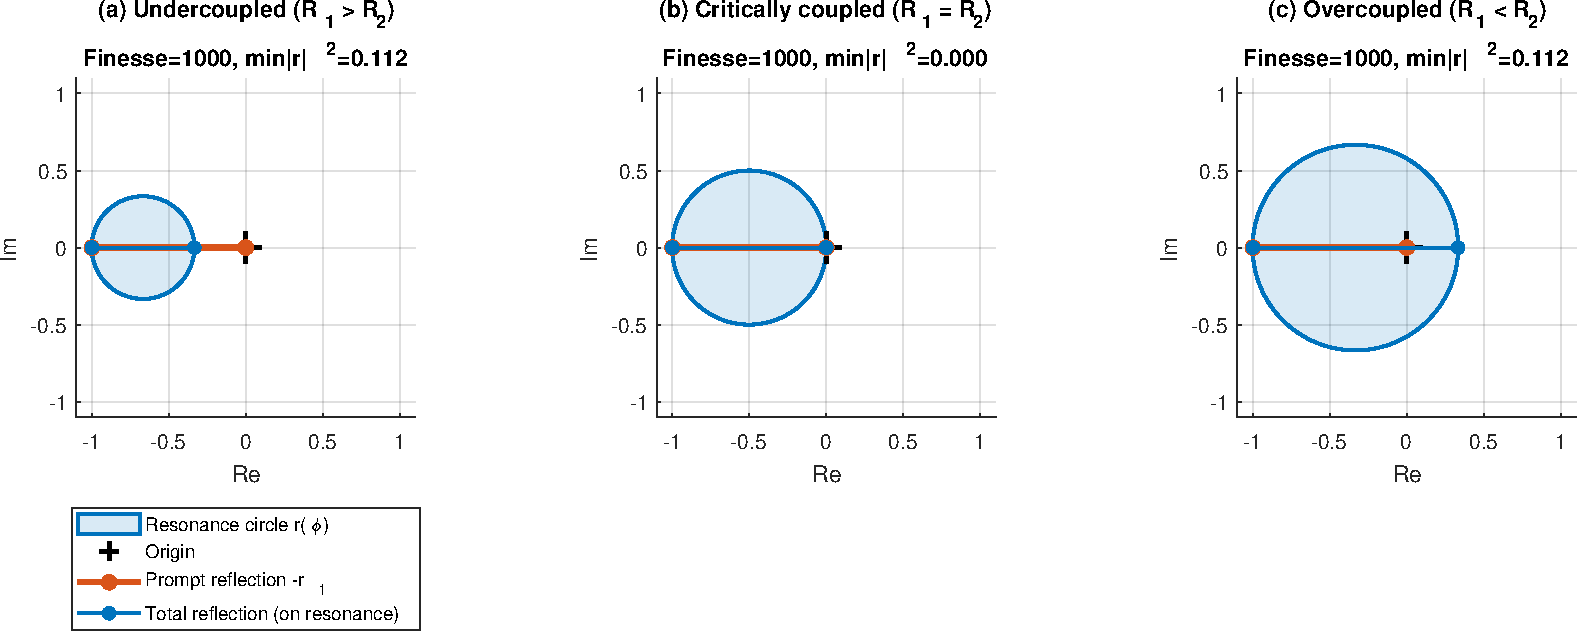
\includegraphics[width=\textwidth]{pic/coupling-regimes.pdf}
\caption{The reflection coefficient's ``resonance circle,'' traced by
$r(\varphi)$ over one full FSR, for an undercoupled, critically coupled, and
overcoupled cavity (same product $r_1 r_2$, hence same Finesse, for panels
(a) and (c) --- only which mirror is called ``front'' has been swapped). The
critically coupled circle (b) passes exactly through the origin. The
undercoupled circle (a) stays entirely outside it. The overcoupled circle
(c) encloses it. On-resonance reflection is decomposed with the same two
colors as Figure~\ref{fig:phasor-chain-conceptual}: orange for the prompt
reflection $-r_1$, blue for the total on-resonance reflection $r(0)$ it sums
to (the net leaked-out contribution, without drawing each round trip) ---
note the blue endpoint sits on the \emph{same} side as $-r_1$ in (a) but the
\emph{opposite} side in (c), despite both having identical $\min|r|^2$, and
lands exactly on the origin in (b).}
\label{fig:coupling-regimes}
\end{figure}
\begin{table}[H]
\centering
\begin{tabular}{@{}lllllc@{}}
\toprule
Regime & $R_1$ & $R_2$ & Finesse & $\min|r|^2$ & Net phase / FSR \\
\midrule
Undercoupled & 0.9979 & 0.9958 & 1000.0 & 0.1114 & $0^\circ$ \\
Critically coupled & 0.9969 & 0.9969 & 1000.0 & 0.0000 & $360^\circ$ \\
Overcoupled & 0.9958 & 0.9979 & 1000.0 & 0.1114 & $360^\circ$ \\
\bottomrule
\end{tabular}

\caption{Minimum reflected power and net accumulated reflection phase over
one full FSR sweep, for the three cavities of
Figure~\ref{fig:coupling-regimes}. Generated by \textit{generateReportFigures.m}
(\textit{exportCouplingRegimesTable}) directly from \textit{OpticalCavity}.}
\label{tab:coupling-regimes}
\end{table}
Table~\ref{tab:coupling-regimes}'s last column makes the circle-enclosure
argument concrete: the net phase accumulated by $r(\varphi)$ over one full
FSR is exactly $360^\circ$ whenever the resonance circle encloses or passes
through the origin (critical and overcoupled), and exactly $0^\circ$ ---
the phasor wobbles back and forth but never completes the loop --- whenever
the origin sits outside it (undercoupled). This is precisely the same
$360^\circ$ phase step already seen in
Figure~\ref{fig:cavity-response}'s Panel~3, for the matched-mirror
(critically coupled) running example.

To see this play out in the same panel layout as Figure~\ref{fig:cavity-response}
rather than only as an abstract circle, Figures~\ref{fig:cavity-response-undercoupled}
and~\ref{fig:cavity-response-overcoupled} reuse \textit{plotCavityResponse.m}
directly for the \textit{ExampleCavities.UndercoupledLowFinesse} and
\textit{ExampleCavities.OvercoupledLowFinesse} fixtures (\S\ref{sec:cavity-coupling}
introduces the full \textit{ExampleCavities} fixture set). The Low-Finesse
tier is used here so the phase's turning behavior is visible within the same
$\pm5$-linewidth window used throughout this report --- the effect exists at
any finesse, since Table~\ref{tab:coupling-regimes} already demonstrated it
numerically for the same fixtures' High-Finesse tier.
\begin{figure}[H]
\centering
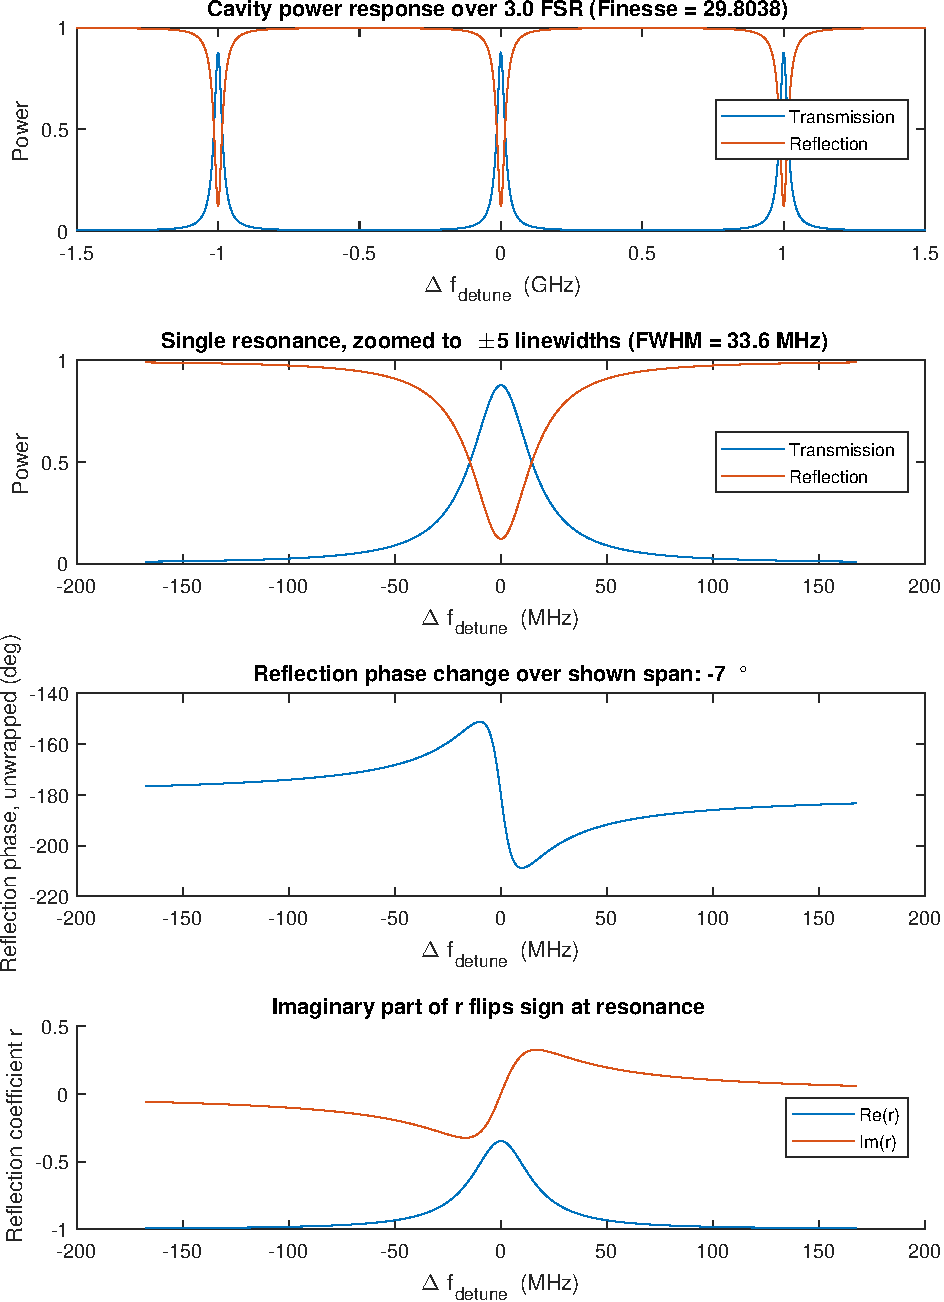
\includegraphics[width=0.75\textwidth]{pic/cavity-response-undercoupled.pdf}
\caption{\textit{plotCavityResponse.m} for \textit{ExampleCavities.UndercoupledLowFinesse}
($R_1=0.9337>R_2=0.8675$, $\mathcal{F}=29.8$). Panel~3 shows the
reflection phase swooping from $-176.6^\circ$ down to a minimum near
$-208.8^\circ$ and turning back toward $-183.4^\circ$ --- never approaching a
monotonic $360^\circ$ sweep; the net change over the shown span is only
$-6.7^\circ$, consistent with the $0^\circ$ full-FSR winding number of
Table~\ref{tab:coupling-regimes}. Panel~4's $\mathrm{Re}(r)$ shows the
corresponding small bump rather than a clean sign crossing, reflecting a
reflection dip that comes close to zero ($\min|r|^2=0.1219$) but never
reaches it.}
\label{fig:cavity-response-undercoupled}
\end{figure}
% CHECKED-BY: ReportClaimsCavityTest.undercoupledResponseFigureMatchesCaptionedNumbers
\begin{figure}[H]
\centering
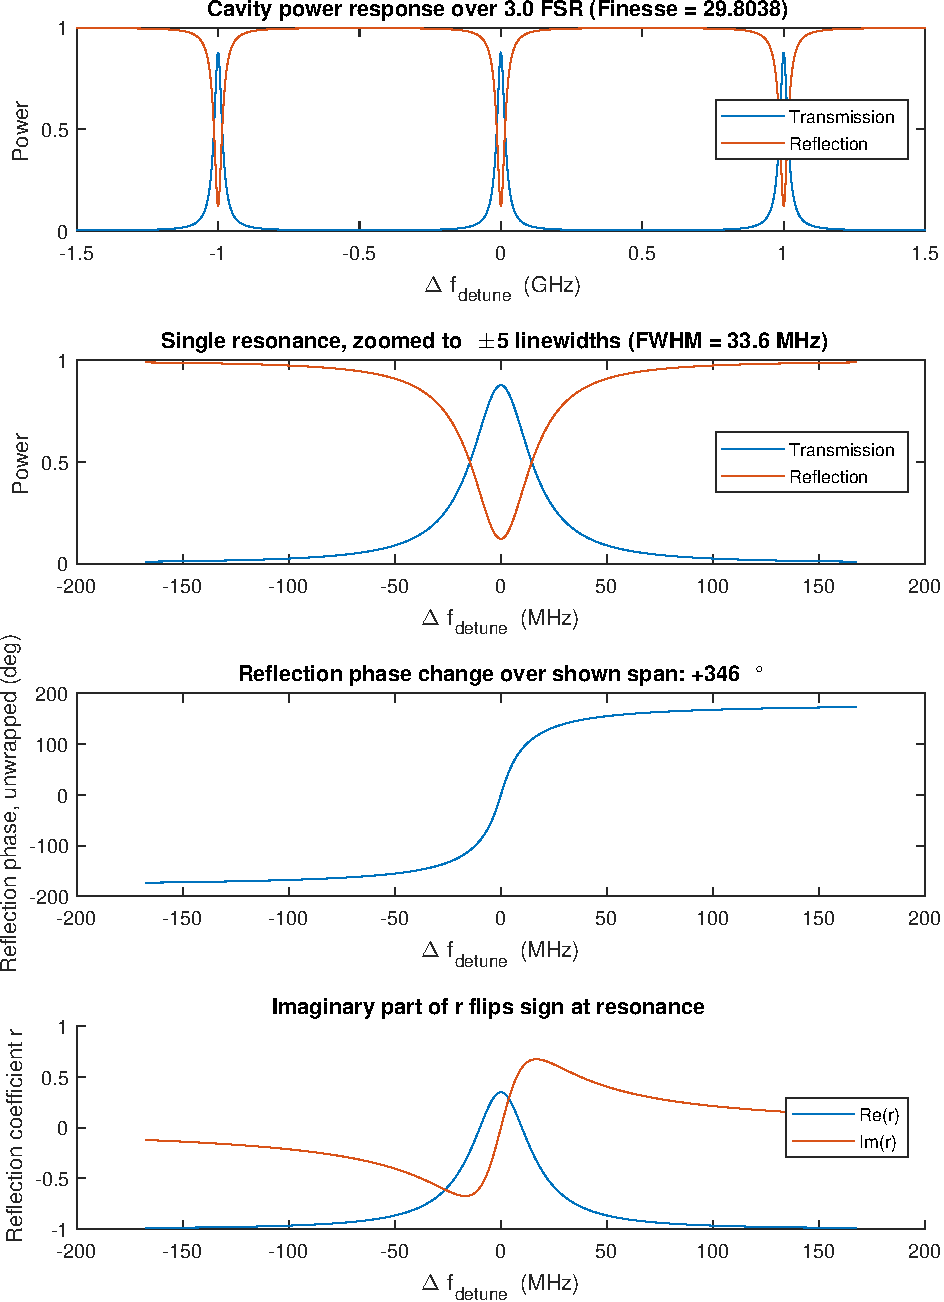
\includegraphics[width=0.75\textwidth]{pic/cavity-response-overcoupled.pdf}
\caption{\textit{plotCavityResponse.m} for \textit{ExampleCavities.OvercoupledLowFinesse}
--- the mirror-swapped counterpart of Figure~\ref{fig:cavity-response-undercoupled}
above ($R_1=0.8675<R_2=0.9337$, the same $\mathcal{F}=29.8$ and the same
$\min|r|^2=0.1219$). Panel~3 shows a clean, nearly monotonic sweep from
$-173.0^\circ$ to $+173.0^\circ$, a net change of $+346.0^\circ$ --- already
most of a full $360^\circ$ revolution within just $\pm5$ linewidths,
confirming the resonance circle's enclosure of the origin. Panel~4's
$\mathrm{Re}(r)$ correspondingly crosses zero, unlike the undercoupled case
above, even though the two cavities' reflection dips are identical in
depth.}
\label{fig:cavity-response-overcoupled}
\end{figure}
% CHECKED-BY: ReportClaimsCavityTest.overcoupledResponseFigureMatchesCaptionedNumbers
This distinction matters directly for PDH: the error signal built in
Section~\ref{sec:sidebands} and later sections is derived entirely from this
reflection phase response. An undercoupled cavity's phase never completes
its excursion, so the resulting error-signal feature is fundamentally
weaker --- a shallow wobble rather than a steep dispersive slope --- even
though its reflected-power dip can look identical to an overcoupled
cavity's. This is why cavities intended for PDH locking are designed to be
critically coupled or overcoupled, never undercoupled: only those two
regimes deliver the full, steep dispersive S-curve that
Figure~\ref{fig:cavity-response}'s Panel~4 and everything built on it
depend on.

\section{Phase Modulation and Sidebands}
\label{sec:sidebands}
\subsection{Why modulate the light at all}
\label{sec:sidebands-motivation}
The photodiode after the cavity can only measure power, the field's squared
magnitude. That throws
away all phase information --- and the whole point of PDH is to recover the
cavity's \emph{phase} response (Section~\ref{sec:cavity-response}, Panels
3--4), which side of resonance the laser sits on, not just its amplitude
response (symmetric, and unable to give a sign).

The trick: put a phase reference onto the light \emph{before} it reaches the
cavity, in the form of sidebands at a known frequency, chosen far
outside the cavity linewidth. Those sidebands pass the cavity essentially
unaffected (they are off-resonance), while the carrier --- if it is close to
resonance --- picks up a cavity-induced phase shift. When carrier and
sidebands recombine on the photodiode, they beat at that frequency, and that
beat note's phase encodes the carrier's phase shift. Demodulating (mixing
down) at the same frequency recovers it as a usable error signal. That
demodulation step is the subject of a later ticket; this section is only
about how the sidebands themselves come to exist.

\subsection{The Jacobi-Anger expansion}
\label{sec:sidebands-derivation}
Phase modulation imprints an oscillating phase term onto the carrier; its
Jacobi-Anger expansion (below) turns that single oscillating phase into a
discrete spectrum of sidebands. Table~\ref{tab:sidebands-glossary} collects
the notation used throughout this section.
\begin{table}[H]
\centering
\small
\begin{tabular}{@{}llp{7cm}@{}}
\toprule
Symbol & Code identifier & Meaning \\
\midrule
$\omega_{\mathrm{laser}}$ & --- & laser (carrier) angular frequency, $\omega_{\mathrm{laser}}=2\pi f_{\mathrm{laser}}$ (the same $f_{\mathrm{laser}}$ of Eq.~\eqref{eq:detuning-def}) \\
$E(t)$, $E_0$ & --- & the modulated field, and its (unmodulated) carrier amplitude (Eq.~\eqref{eq:pm-field}) \\
$\beta$ & \textit{modulationIndex} & phase modulation depth, radians \\
$\omega_m$, $f_m$ & \textit{modulationFrequencyHz} & modulation (angular) frequency \\
$J_\ell(\beta)$ & \textit{sidebands.Amplitude} & Bessel-function sideband amplitude at order $\ell$ \\
$\ell$ & \textit{sidebands.Order} & sideband order, $\ell=-\mathrm{MaxOrder}\ldots\mathrm{MaxOrder}$ \\
$\mathcal{E}_\ell$ & --- & phasor amplitude of spectral line $\ell$ ($\ell=-1,0,1$), $\equiv J_\ell(\beta)$ (Eq.~\eqref{eq:sidebands-phasor-amplitude}); $\mathcal{E}_{-1}=-\mathcal{E}_1$ \\
\addlinespace
\multicolumn{3}{@{}l}{\textit{IQ modulator (\S\ref{sec:sidebands-iq-modulator}): subscript convention and arm labels}} \\
$(\cdot)_{I,Q}$ & --- & subscript convention, applied to several symbols below: ``the same equation holds once with $I$ throughout, once with $Q$ throughout'' --- never a third, separate quantity of its own \\
$I$, $Q$ (as arm labels) & --- & positional labels for the two arms --- never used bare for the demodulation-phase I/Q Quadrature choice of a later section (\texttt{CONTEXT.md}) \\
\addlinespace
\multicolumn{3}{@{}l}{\textit{IQ modulator: electric fields}} \\
$E_{\mathrm{out}}(t)$ & --- & the IQ modulator's own output field (Eq.~\eqref{eq:iqm-envelope}) \\
$s_{I,Q}(t)$; $s_I(t)$, $s_Q(t)$ & \textit{inPhase}, \textit{quadrature} & each arm's own real, signed field-amplitude coefficient (dimensionless, normalized to $E_0$), defined by Eq.~\eqref{eq:iqm-mzm-transfer}/\eqref{eq:iqm-null-bias}; \emph{not} a voltage (contrast $V_{I,Q}(t)$ below) \\
\addlinespace
\multicolumn{3}{@{}l}{\textit{IQ modulator: biases and drive voltages}} \\
$\theta_{\mathrm{IQ}}$ & --- & the parent combiner's own inter-arm bias (radians), nominally $\pi/2$, trimmed to compensate its manufacturing tolerance (Eq.~\eqref{eq:iqm-envelope}) \\
$V_\pi$, $V_{\pi,I,Q}$ & --- & modulator half-wave voltage (Eq.~\eqref{eq:iqm-vpi}): the drive voltage that shifts one MZM's phase by $\pi$; generic, single-device form \\
$V_{\pi,I}$, $V_{\pi,Q}$ & --- & each arm's own independently-set half-wave bias --- Eq.~\eqref{eq:iqm-vpi} predicts them equal only if both arms' crystal parameters match exactly, which real fabrication does not guarantee \\
$V_{I,Q}(t)$; $V_I(t)$, $V_Q(t)$ & --- & a single arm's total drive voltage, bias plus RF (Eq.~\eqref{eq:iqm-drive-voltage}) \\
$v_{I,Q}(t)$; $v_I(t)$, $v_Q(t)$ & --- & the RF (small-signal) part of $V_{I,Q}(t)$ layered on top of its bias: $v_{I,Q}(t)=V_{I,Q}(t)-V_{\pi,I,Q}$ \\
\addlinespace
\multicolumn{3}{@{}l}{\textit{IQ modulator: Pockels cell (material/geometry constants)}} \\
$n_e$, $r_{33}$, $d$, $L_{\mathrm{mod}}$ & --- & extraordinary refractive index, electro-optic coefficient, electrode gap, interaction length (Eq.~\eqref{eq:iqm-pockels}) --- $L_{\mathrm{mod}}$ deliberately not written $L$, to avoid colliding with Section~\ref{sec:cavity}'s cavity length \\
$\Delta n_e(V)$ & --- & Pockels-effect perturbation of $n_e$ under a generic applied voltage $V$ (Eq.~\eqref{eq:iqm-pockels}) \\
$\Delta\phi(V)$ & --- & voltage-controlled phase shift of a single MZM sub-path under $V$ (Eq.~\eqref{eq:iqm-phase-shift}) \\
\bottomrule
\end{tabular}
\caption{Notation used throughout Section~\ref{sec:sidebands}.}
\label{tab:sidebands-glossary}
\end{table}
The field leaving the electro-optic modulator (EOM) is
\begin{equation}
E(t) = E_0\, e^{i(\omega_{\mathrm{laser}} t + \beta \sin\omega_m t)},
\label{eq:pm-field}
\end{equation}
where $\omega_{\mathrm{laser}} = 2\pi f_{\mathrm{laser}}$ is the laser's own
angular frequency --- the same $f_{\mathrm{laser}}$ introduced alongside
detuning in Eq.~\eqref{eq:detuning-def}, just in angular rather than linear
units; it is deliberately not written $\omega_0$, to avoid colliding with
Section~\ref{sec:cavity}'s unrelated use of the subscript $0$ for a
resonance's mode number ($f_{0,N}$, Eq.~\eqref{eq:mode-comb}). With
modulation index $\beta$ (how many radians of phase are being wobbled) and
modulation angular frequency $\omega_m = 2\pi f_m$, factoring out the
fast carrier oscillation and expanding what is left using the Jacobi-Anger
identity,
\begin{equation}
e^{i\beta\sin\omega_m t} = \sum_{\ell=-\infty}^{\infty} J_\ell(\beta)\, e^{i\ell\omega_m t},
\label{eq:jacobi-anger}
\end{equation}
which is an \emph{identity}, not an approximation --- the approximation only
enters when the sum is truncated. Each term $\ell$ is a sideband at frequency
$\omega_{\mathrm{laser}} + \ell\omega_m$, weighted by the Bessel function $J_\ell(\beta)$.
\textit{generatePhaseModulationSidebands.m} computes exactly this table of
coefficients (\verb|besselj(order, modulationIndex)|) for
$\ell=-\mathrm{MaxOrder}\ldots\mathrm{MaxOrder}$.

Keeping only $\ell\in\{-1,0,+1\}$ (the project's \textit{MaxOrder}$=1$ default):
\begin{equation}
E(t) \approx E_0\left[J_0(\beta) + J_1(\beta)\,e^{i\omega_m t} + J_{-1}(\beta)\,e^{-i\omega_m t}\right]e^{i\omega_{\mathrm{laser}} t}.
\label{eq:pm-truncated}
\end{equation}
The identity $J_{-1}(\beta) = -J_1(\beta)$ (odd-order Bessel functions are odd
functions of their order) is not a detail --- it is the entire reason phase
modulation looks different from amplitude modulation in the phasor picture.
Substituting it into Eq.~\eqref{eq:pm-truncated} and using Euler's formula:
\begin{equation}
J_0(\beta) + J_1(\beta)\left[e^{i\omega_m t} - e^{-i\omega_m t}\right]
= J_0(\beta) + i\, 2 J_1(\beta) \sin(\omega_m t).
\label{eq:pm-real-imag}
\end{equation}
The real part stays pinned at $J_0(\beta)$; the imaginary part swings back
and forth as $2J_1(\beta)\sin(\omega_m t)$. In the complex plane, the
resultant phasor does not trace a circle (that would be amplitude
modulation) --- it wiggles up and down along a vertical line centered on the
real axis. That vertical wiggle \emph{is} phase modulation: since
$\arg(E) \approx \frac{2J_1(\beta)}{J_0(\beta)}\sin(\omega_m t)$ for small
deviations, the phase angle oscillates while the magnitude stays almost
exactly $J_0(\beta)$ --- exactly constant only if the full infinite sum of
Eq.~\eqref{eq:jacobi-anger} is kept. At $\beta=1.08$, $J_0(1.08)=0.7281$,
$J_1(1.08)=0.4656$, and truncating at $\ell=\pm1$ reproduces the exact field
of Eq.~\eqref{eq:pm-field} to within about $27\%$ at the extremes of the
cycle --- the size of the next dropped term, $J_2(1.08)\approx0.1326$,
doubled for the pair $\ell=\pm2$, considerably rougher than the truncation
would be at a smaller modulation depth. Section~\ref{sec:sidebands-regimes}
returns to why this particular $\beta$ is used here, and to the
higher-order sidebands this truncation drops.
% CHECKED-BY: ReportClaimsSidebandsTest.besselCoefficientsInJacobiAngerWorkedExample

\subsection{Amplitude scaling with modulation depth}
\label{sec:sidebands-regimes}
Eq.~\eqref{eq:jacobi-anger} says more than ``there are sidebands'': each
sideband's amplitude $J_\ell(\beta)$ is a specific, computable function of
the modulation index, so raising or lowering $\beta$ redistributes field
amplitude between the carrier and the sidebands in a definite way, not just
a vague ``more modulation, more sidebands.'' Figure~\ref{fig:sideband-regimes}
plots the carrier and the $\ell=\pm1,\pm2,\pm3$ sidebands as vertical lines
at four representative values of $\beta$ (\textit{ExampleModulationRegimes}),
spanning what this project calls the Modulation Regimes.
\begin{figure}[H]
\centering
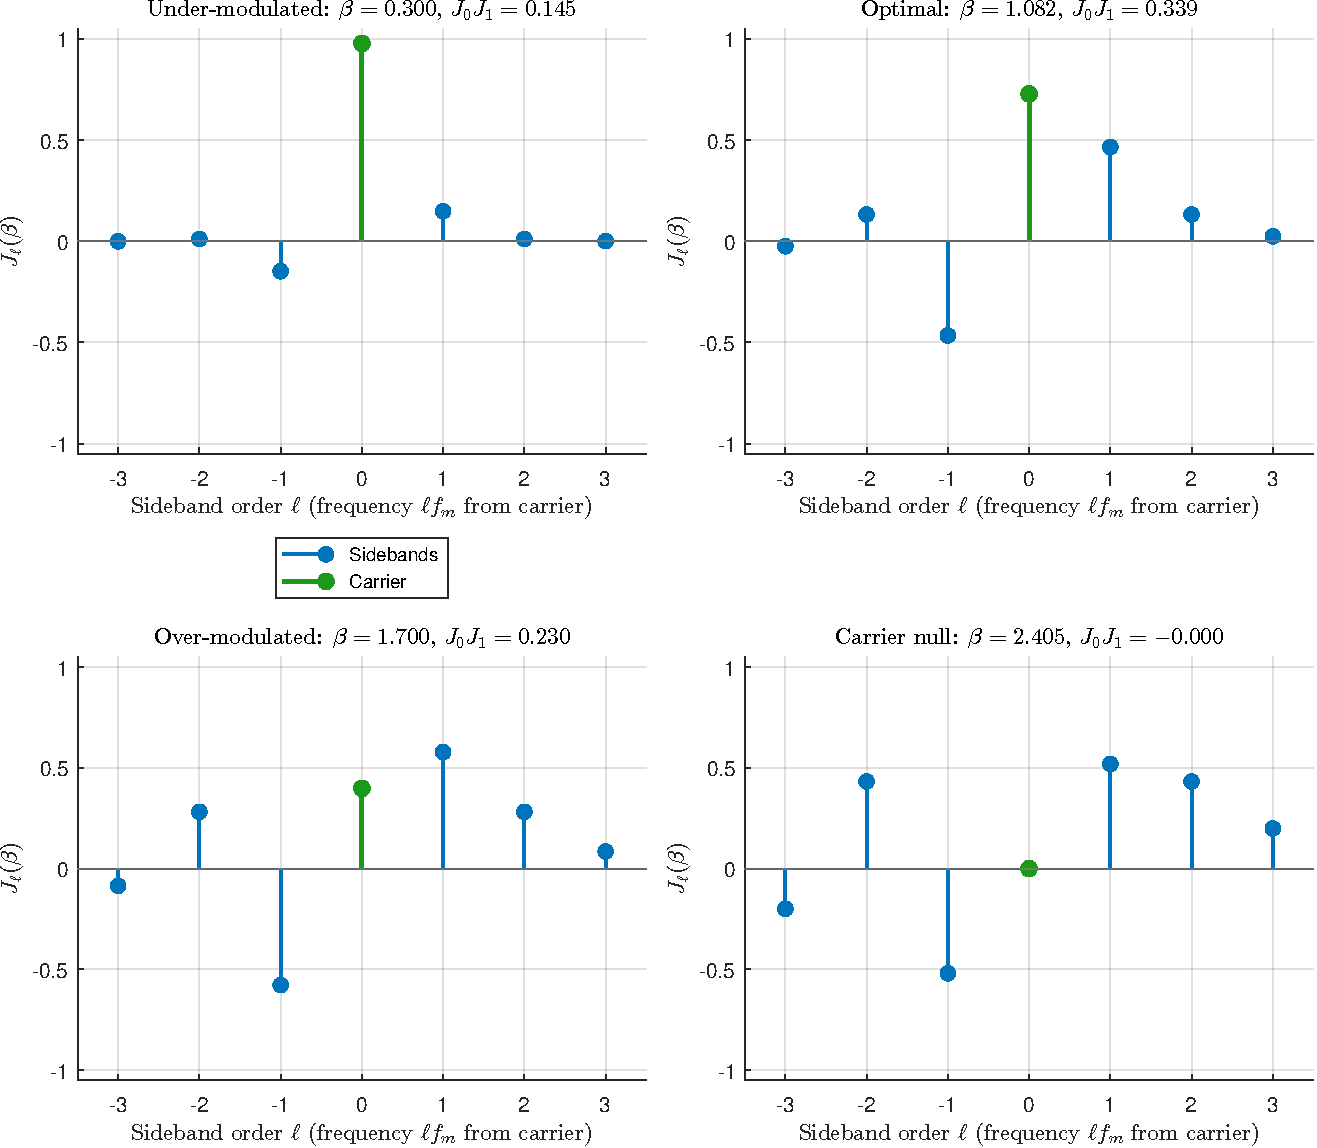
\includegraphics[width=\textwidth]{pic/sideband-regimes.pdf}
\caption{Carrier (green) and sideband (blue) field amplitudes $J_\ell(\beta)$
vs.\ sideband order $\ell$, at the four \textit{ExampleModulationRegimes}
values. Under-modulated ($\beta=0.3$): almost all the field stays in the
carrier. Optimal ($\beta\approx1.08$, this project's running example): the
carrier/sideband amplitude product $J_0(\beta)J_1(\beta)$ is maximized.
Over-modulated ($\beta=1.7$): field has moved past the optimum into
higher-order sidebands, and the product has fallen again. Carrier null
($\beta=2.4048$, the first zero of $J_0$): the carrier line vanishes
entirely.}
\label{fig:sideband-regimes}
\end{figure}
At $\beta=0.3$ (\textbf{under-modulated}), the carrier line towers over
sidebands that are barely visible above the axis: most of the field
amplitude never left the carrier. Raising $\beta$ moves amplitude out of the
carrier and into the sidebands --- visibly so between the first two panels
--- but not without limit: past $\beta\approx1.08$ (\textbf{over-modulated}),
the carrier keeps shrinking while the amount landing in the $\ell=\pm1$
sidebands specifically (as opposed to higher orders) starts shrinking too,
spreading out into $\ell=\pm2,\pm3$ instead. Pushed far enough, at
$\beta=2.4048$ the carrier line disappears altogether (\textbf{carrier
null}, the first zero of $J_0$) --- all of the original carrier amplitude
has been redistributed among the sidebands.

The value $\beta\approx1.08$~rad already used, unexplained, in the worked
example of \S\ref{sec:sidebands-derivation} is not arbitrary. Why does it
matter specifically, rather than ``more sidebands are always better''?
Section~\ref{sec:sidebands-motivation} already named the mechanism the rest
of this report builds on: carrier and
sidebands eventually recombine on a photodiode and \emph{beat} against each
other, and it is that beat note's phase that carries the cavity's response.
A beat note needs both parties present in some amount --- an
undetectably small sideband has nothing to beat against, however cleanly
phase-shifted the carrier becomes, and an undetectably small carrier is
equally useless however strong the sidebands are. That is why the relevant
quantity is not $J_1(\beta)$ alone (which keeps growing well past
$\beta=1.08$, not peaking until $\beta\approx1.8$) but the \emph{product}
$J_0(\beta)J_1(\beta)$: it has an interior maximum precisely because growing
one factor eventually costs more in the other than it gains. This report
does not yet derive the demodulated PDH error signal itself (that is the
subject of the next sections), but the same product sets its slope, which
is why $\beta\approx1.08$~rad --- maximizing $J_0(\beta)J_1(\beta)$ at
$\approx0.339$, more than double the under-modulated regime's $0.145$ --- is
the standard choice quoted in the literature \cite{black2001pdh} for getting the
strongest possible PDH signal out of a given amount of laser power.
% CHECKED-BY: ReportClaimsSidebandsTest.optimalModulationDepthMaximizesCarrierSidebandProduct
% CHECKED-BY: ReportClaimsSidebandsTest.carrierNullIsFirstZeroOfJ0

That maximum, though, is a maximum of the $\ell=\pm1$ content alone --- and
\S\ref{sec:sidebands-derivation}'s worked example already showed that at
$\beta\approx1.08$ the $\ell=\pm1$ truncation itself is a rough
approximation, because $\ell=\pm2$ and higher are no longer negligible
(Figure~\ref{fig:sideband-regimes}, third and fourth panels). Is there a way
to modulate the carrier without also populating these higher orders? Not
with a single EOM driven at one tone: Eq.~\eqref{eq:jacobi-anger} is an
identity, so for any nonzero $\beta$ every order $\ell$ has a nonzero
$J_\ell(\beta)$, and there is no separate knob that turns off $\ell=\pm2$
while leaving $\ell=\pm1$ alone --- $\beta$ is the only free parameter, and
it sets the whole spectrum at once. What does change with $\beta$ is how
much of the total field ends up beyond first order: for small $\beta$,
$J_\ell(\beta)\approx\frac{1}{\ell!}(\beta/2)^{|\ell|}$, so each higher order
is suppressed by an extra power of $\beta$ relative to the last. The ratio
$J_2(\beta)/J_1(\beta)$ makes this concrete: $7.5\%$ at the under-modulated
$\beta=0.3$, $28.5\%$ at the optimal $\beta\approx1.08$, and $48.8\%$ at the
over-modulated $\beta=1.7$ --- which is exactly why real PDH setups often
deliberately run somewhat below the strict $J_0(\beta)J_1(\beta)$ optimum,
trading a little error-signal slope for a spectrum where the ignored higher
orders stay small.
% CHECKED-BY: ReportClaimsSidebandsTest.secondOrderToFirstOrderRatioAcrossRegimes

The higher orders are not, on their own, harmful to the eventual error
signal the way an over-modulated carrier is. Since $f_m$ is chosen far
outside the cavity linewidth (\S\ref{sec:sidebands-motivation}), $\ell=\pm2,
\pm3,\ldots$ sit even further from resonance than $\ell=\pm1$ and come back
from the cavity essentially as untouched as the first-order sidebands do.
What they cost is optical power diverted away from the carrier and
first-order sidebands that actually carry the usable beat note, plus extra
beat terms between adjacent higher orders that add a roughly
detuning-independent background to the demodulated signal rather than a
resonance feature --- a nuisance to filter around, not a corruption of the
signal's shape (the full argument needs the demodulation math of the next
sections). A dedicated narrowband optical filter placed after the EOM could
reject them outright, since they sit at clean integer multiples of $f_m$,
but this is rarely done in practice --- backing off $\beta$ a little is
simpler, and, as the ratios above show, already suppresses them
geometrically.

\subsection{The phasor picture}
\label{sec:sidebands-phasors}
\begin{figure}[H]
\centering
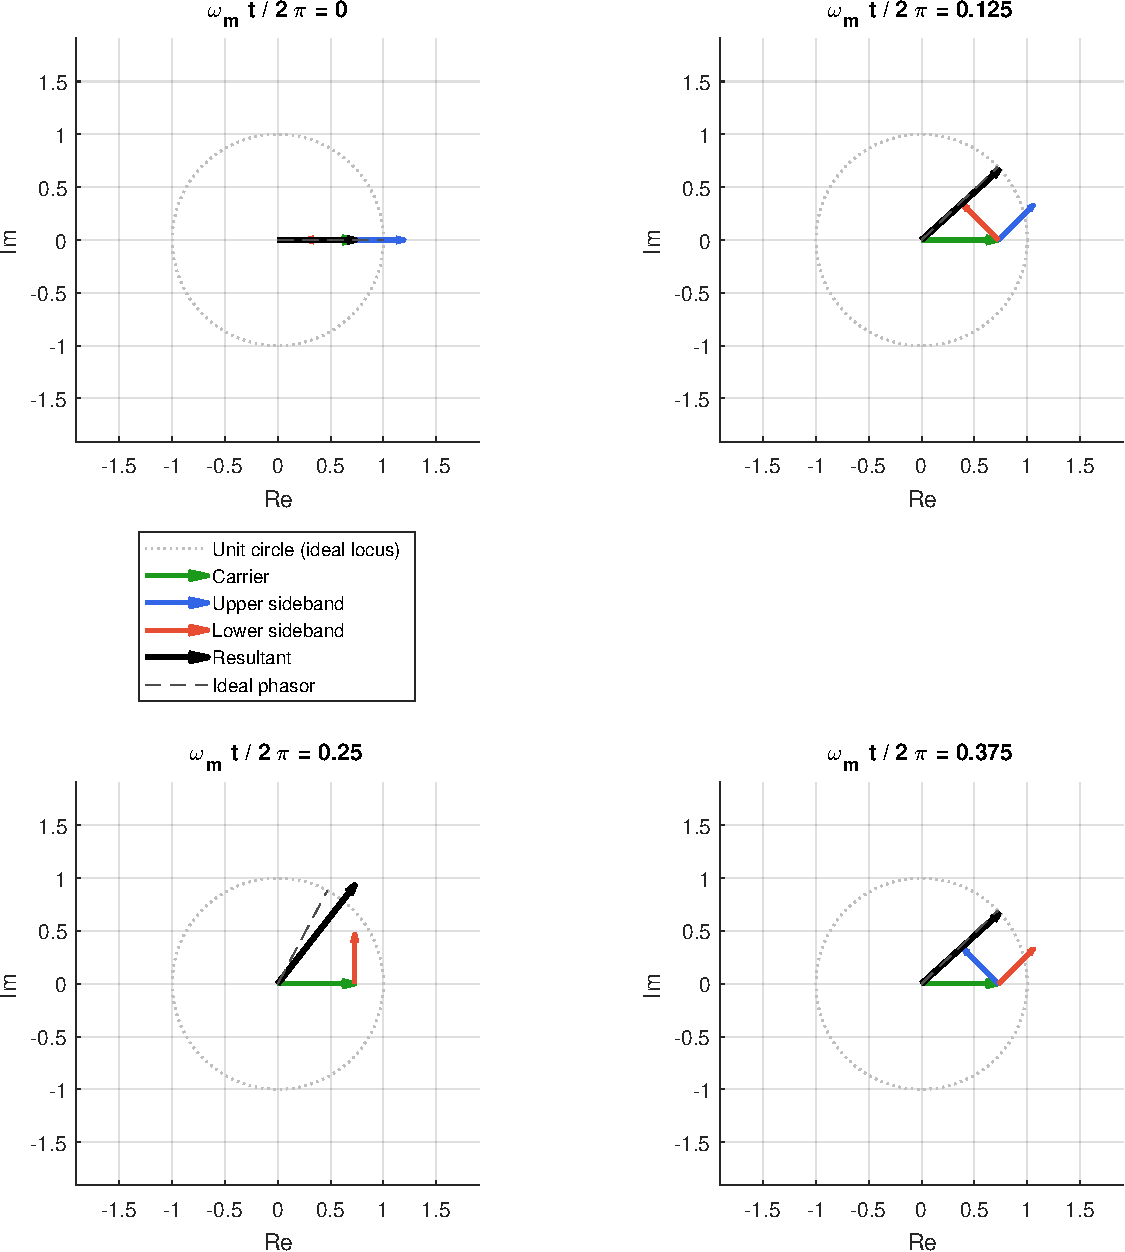
\includegraphics[width=0.8\textwidth]{pic/phasor-snapshots.pdf}
\caption{Four snapshots across one modulation cycle of the carrier +
sideband phasor picture (a static stand-in for the live animation in
\textit{animatePhaseModulatedPhasors.m}), at $\beta\approx1.08$ (Optimal
Modulation Depth, \S\ref{sec:sidebands-regimes}),
$f_m=\SI{15}{\mega\hertz}$. Green: carrier, fixed (the frame co-rotates with
it). Blue/red: upper/lower sideband, drawn starting at the carrier's tip,
rotating at $\pm\omega_m$. Black: the true resultant. Dashed grey: the exact
(infinite-order) phasor $e^{i\beta\sin\omega_m t}$ at this instant. Dotted
light grey: the full unit circle that exact phasor traces over the whole
cycle --- radius exactly $1$, since pure phase modulation changes only
$\arg(E)$, never $|E|$.}
\label{fig:phasor-snapshots}
\end{figure}
Figure~\ref{fig:phasor-snapshots} draws exactly the three-phasor picture of
Eq.~\eqref{eq:pm-truncated}, in the frame rotating with the carrier (so the
carrier itself sits still). The sideband arrows are drawn starting at the
tip of the carrier arrow, not at the origin, so their vector sum relative to
that tip is visible directly as the thing that makes the resultant wobble.

Name each arrow's own complex amplitude explicitly, since later sections
(the cavity's effect on each line, \S\ref{sec:pdh-photodiode}, and the
dot-product construction of \S\ref{sec:pdh-dotproduct}) need to refer to it
directly rather than re-deriving it from the Jacobi-Anger expansion each
time:
\begin{equation}
\mathcal{E}_\ell \equiv J_\ell(\beta), \qquad \ell\in\{-1,0,1\},
\label{eq:sidebands-phasor-amplitude}
\end{equation}
the carrier's own phasor amplitude $\mathcal{E}_0$ (green) and the
upper/lower sideband phasor amplitudes $\mathcal{E}_{\pm1}$ (blue/red) of
Eq.~\eqref{eq:pm-truncated} --- with $\mathcal{E}_{-1}=-\mathcal{E}_1$
inherited directly from $J_{-1}(\beta)=-J_1(\beta)$, the same odd-order
identity already used to reach Eq.~\eqref{eq:pm-real-imag}.

The light grey dotted circle is not a visual approximation: pure phase
modulation changes only the phasor's angle, never its length, so the exact
field $E(t)/E_0=e^{i\beta\sin\omega_m t}$ has $|E(t)/E_0|=1$ for every $t$,
exactly, regardless of $\beta$ --- because $|e^{i\theta}|=1$ for any real
$\theta$, and $\beta\sin\omega_m t$ is always real. Amplitude modulation
would instead change the radius and leave the angle alone; phase modulation
does the opposite, which is why the exact phasor traces this particular
circle, of radius exactly $1$ and not merely close to it, rather than some
other curve.

Two things to check across the four panels:

\begin{enumerate}
\item \textbf{The counter-rotation itself.} At every instant, the upper
sideband's angle and the lower sideband's angle are reflections of each
other through the horizontal: one is $e^{+i\omega_m t}$, the other
$e^{-i\omega_m t}$ --- same speed, opposite direction. This is a direct
consequence of $J_{-1}(\beta)=-J_1(\beta)$; a symmetric spectrum
($J_{-1}=+J_1$, as in amplitude modulation) would instead have both
sidebands co-rotating.
\item \textbf{Why counter-rotation turns into a vertical wobble, not a
circular motion.} At $t=0$ (top-left panel) both sideband arrows point along
the real axis in opposite directions and exactly cancel: the resultant sits
right on the carrier's tip, no wobble yet. As $t$ advances (remaining
panels), the two arrows swing away from the real axis in mirrored
directions, so their real components stay matched (still canceling) while
their imaginary components both grow the same way --- precisely
Eq.~\eqref{eq:pm-real-imag}.
\end{enumerate}

At this modulation depth the resultant (black) departs visibly from the
dotted unit circle in both directions across the wobble --- dipping inside
to $|J_0(\beta)|\approx0.73$ at $t=0$ (top-left panel) and bulging outside
to $\approx1.18$ at the wobble's peak (bottom-left panel) --- instead of
merely grazing it the way a smaller $\beta$ would. Both excursions are the
same $\approx27\%$ truncation error from keeping only $\ell=0,\pm1$, the one
quantified numerically at the end of Section~\ref{sec:sidebands-derivation}.
% CHECKED-BY: ReportClaimsSidebandsTest.phasorResultantMagnitudeExcursionsAtOptimalModulationDepth

\subsection{Synthesizing the sidebands with an IQ modulator}
\label{sec:sidebands-iq-modulator}
Section~\ref{sec:sidebands-regimes} asked whether the higher orders could be
switched off without also killing $\ell=\pm1$, and found no such knob on a
single EOM: $\beta$ is its only free parameter, and Eq.~\eqref{eq:jacobi-anger}
being an identity means it sets every order at once. An \emph{IQ modulator}
answers the same question differently, by replacing one nonlinearly-driven
waveguide with two independently-biased ones, combined in quadrature.

This subsection derives $E_{\mathrm{out}}(t)$ as an explicit function of
five independent inputs --- three biases ($V_{\pi,I}$, $V_{\pi,Q}$,
$\theta_{\mathrm{IQ}}$) and two time-varying drive voltages ($v_I(t)$,
$v_Q(t)$) --- plus the Pockels cell's own material/geometry constants
($n_e$, $r_{33}$, $d$, $L_{\mathrm{mod}}$, and $\lambda$ shared with
Section~\ref{sec:cavity}). Every intermediate quantity along the way gets
its own equation, in order, so the chain from those inputs to
$E_{\mathrm{out}}(t)$ has no unstated step.

\textbf{The physics: a crystal, not a circuit.} Both a phase-modulating EOM
(Eq.~\eqref{eq:pm-field}) and an IQ modulator exploit the same underlying
effect: the linear electro-optic (Pockels) effect in a non-centrosymmetric
crystal such as lithium niobate (LiNbO$_3$). Applying a voltage $V$ across
electrodes patterned alongside a waveguide linearly perturbs the crystal's
own (extraordinary) refractive index,
\begin{equation}
\Delta n_e(V) = -\tfrac{1}{2}n_e^3 r_{33}\frac{V}{d},
\label{eq:iqm-pockels}
\end{equation}
where $r_{33}$ is the relevant electro-optic coefficient and $d$ the
electrode gap --- solid-state physics of a specific kind: a bulk dielectric
crystal's own birefringence, tuned by an applied field, with no free
carriers or semiconductor band structure involved (unlike, say, an
electro-absorption modulator), which is also why it is fast: nothing has to
move except the light itself. Over an interaction length $L_{\mathrm{mod}}$,
Eq.~\eqref{eq:iqm-pockels} becomes a voltage-controlled phase shift,
\begin{equation}
\Delta\phi(V) = \frac{2\pi}{\lambda}\Delta n_e(V)\,L_{\mathrm{mod}},
\label{eq:iqm-phase-shift}
\end{equation}
and the half-wave voltage $V_\pi$ --- the drive voltage that shifts phase by
exactly $\pi$ --- is defined by $|\Delta\phi(V_\pi)|=\pi$ in
Eq.~\eqref{eq:iqm-phase-shift}, i.e.
\begin{equation}
V_\pi = \frac{\lambda\,d}{n_e^3\,r_{33}\,L_{\mathrm{mod}}}.
\label{eq:iqm-vpi}
\end{equation}
Eq.~\eqref{eq:iqm-phase-shift} is exactly what a phase-modulating EOM
applies directly to the beam, with $V(t)\propto\sin\omega_m t$ reproducing
Eq.~\eqref{eq:pm-field}'s $\beta\sin\omega_m t$. An IQ modulator instead uses
it as a building block, one level down --- and, since a device's two arms
are two physically separate crystal regions, Eq.~\eqref{eq:iqm-vpi} predicts
the \emph{same} $V_\pi$ for both only if $n_e$, $d$, $L_{\mathrm{mod}}$
match between them exactly. Real fabrication does not hold that tightly,
which is exactly why $V_{\pi,I}$ and $V_{\pi,Q}$ (below) are supplied as two
independently-set bias inputs rather than computed from
Eq.~\eqref{eq:iqm-vpi} at run time.

\textbf{From phase shift to intensity: one child Mach-Zehnder modulator per
arm.} A single Mach-Zehnder modulator (MZM) splits the light into two
sub-paths, drives them push-pull (one gets $+V(t)/2$, the other $-V(t)/2$,
so no common phase --- no chirp --- survives the recombination), and
interferes them back together. Writing this once for either arm (subscript
$I,Q$ meaning ``the same equation holds with $I$ throughout, and again with
$Q$ throughout''), the relative phase from Eq.~\eqref{eq:iqm-phase-shift}
becomes a real, signed field-amplitude coefficient
\begin{equation}
s_{I,Q}(t) \equiv \cos\!\left(\frac{\pi V_{I,Q}(t)}{2V_{\pi,I,Q}}\right),
\label{eq:iqm-mzm-transfer}
\end{equation}
a nonlinear ``raised-cosine'' transfer curve in the arm's own total drive
voltage $V_{I,Q}(t)$ --- bias plus RF, defined next.

\textbf{Biasing at the null: where ``bias'' and ``RF in'' come from.} Each
arm's total drive voltage is its own fixed bias plus a time-varying RF part,
\begin{equation}
V_{I,Q}(t) = V_{\pi,I,Q} + v_{I,Q}(t),
\label{eq:iqm-drive-voltage}
\end{equation}
i.e., explicitly, $V_I(t)=V_{\pi,I}+v_I(t)$ and $V_Q(t)=V_{\pi,Q}+v_Q(t)$.
Substituting Eq.~\eqref{eq:iqm-drive-voltage} into
Eq.~\eqref{eq:iqm-mzm-transfer} --- biasing at the transfer curve's own field
null, $V_{I,Q}=V_{\pi,I,Q}$, not the power-quadrature point $V_{\pi,I,Q}/2$
sometimes used for unipolar analog links --- gives an \emph{exact} identity,
not an approximation:
\begin{equation}
s_{I,Q}(t) = \sin\!\left(\frac{\pi v_{I,Q}(t)}{2V_{\pi,I,Q}}\right)
\approx \frac{\pi v_{I,Q}(t)}{2V_{\pi,I,Q}} \quad (|v_{I,Q}(t)|\ll V_{\pi,I,Q}),
\label{eq:iqm-null-bias}
\end{equation}
linear (in the small-signal limit only), bipolar, and passing through zero
at $v_{I,Q}=0$ --- exactly the shape needed to represent a signed real drive
amplitude; the sign shown is a choice of which electrode is driven positive,
flipped by wiring the electrodes the other way. $V_{\pi,I,Q}$ is the
\emph{bias} Figure~\ref{fig:iq-modulator-schematic} labels; $v_{I,Q}(t)$ is
the \emph{RF in} next to it, superimposed on top. Written out explicitly for
each arm on its own --- the two equations this subsection is named for ---
\begin{equation}
s_I(t) = \sin\!\left(\frac{\pi v_I(t)}{2V_{\pi,I}}\right), \qquad
s_Q(t) = \sin\!\left(\frac{\pi v_Q(t)}{2V_{\pi,Q}}\right).
\label{eq:iqm-drive-explicit}
\end{equation}
\begin{figure}[H]
\centering
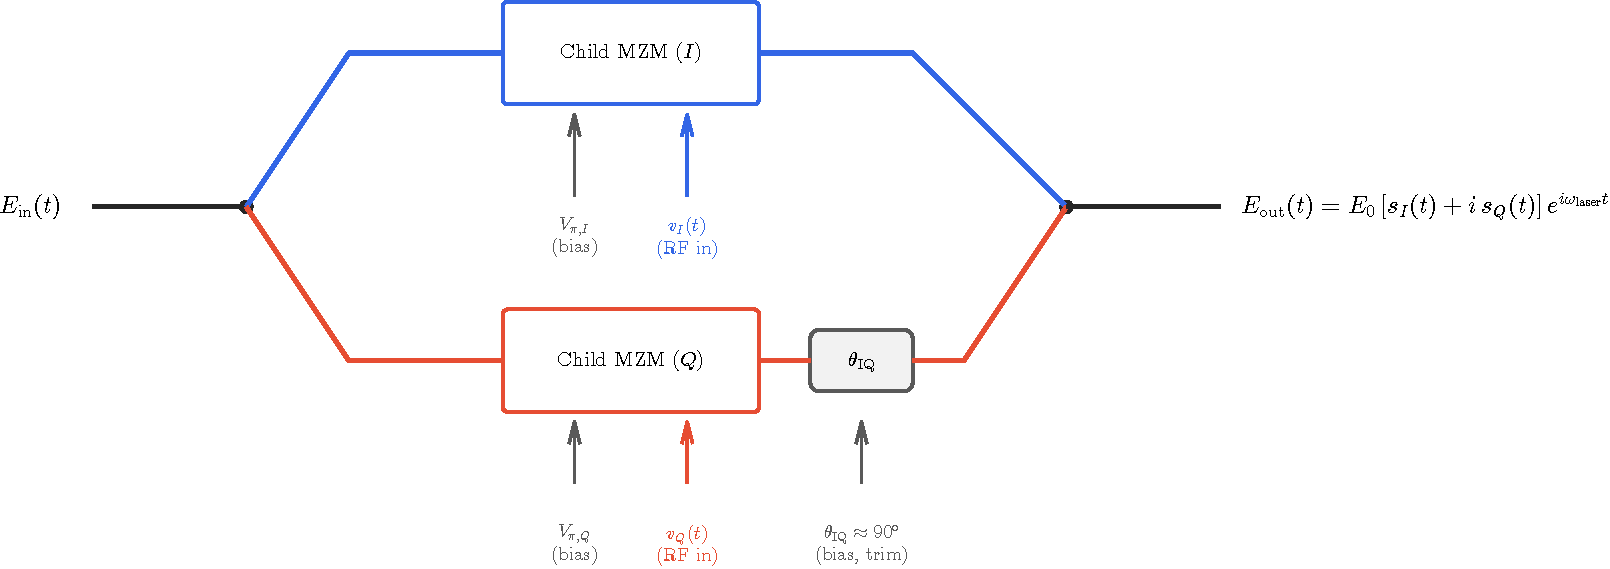
\includegraphics[width=0.95\textwidth]{pic/iq-modulator-schematic.pdf}
\caption{Dual-parallel Mach-Zehnder IQ modulator, schematically. Input light
splits into an $I$-arm (blue) and a $Q$-arm (red), each carrying its own
child MZM (Eq.~\eqref{eq:iqm-mzm-transfer}) with its own bias $V_{\pi,I,Q}$
and RF input $v_{I,Q}(t)$ (Eqs.~\eqref{eq:iqm-drive-voltage}--\eqref{eq:iqm-drive-explicit});
the $Q$-arm then passes through a third, independently trimmable bias
$\theta_{\mathrm{IQ}}\approx90^\circ$ (compensating the parent combiner's own
manufacturing tolerance, not shown to scale) before the two arms recombine
(Eq.~\eqref{eq:iqm-envelope}).}
\label{fig:iq-modulator-schematic}
\end{figure}

\textbf{Two arms in quadrature: the complex output field.} The two arms'
field-amplitude coefficients $s_I(t)$, $s_Q(t)$ (Eq.~\eqref{eq:iqm-drive-explicit})
recombine through a \emph{third}, independent bias, $\theta_{\mathrm{IQ}}$,
applied to the $Q$-arm alone:
\begin{equation}
E_{\mathrm{out}}(t) = E_0\left[s_I(t) + e^{i\theta_{\mathrm{IQ}}}\,s_Q(t)\right]e^{i\omega_{\mathrm{laser}}t},
\qquad \theta_{\mathrm{IQ}} = \frac{\pi}{2} \text{ (nominal)},
\label{eq:iqm-envelope}
\end{equation}
absorbing the arms' static splitting/recombining loss into $E_0$'s own
normalization, the same way this report already leaves such constant
prefactors out of $E_0$ elsewhere. Unlike $V_{\pi,I}$/$V_{\pi,Q}$ (which each
linearize \emph{one arm's own} amplitude response, Eq.~\eqref{eq:iqm-null-bias}),
$\theta_{\mathrm{IQ}}$ sets the angle \emph{between} the two arms and carries
no amplitude information at all. It is also not fixed by geometry the way
the nominal value $\pi/2$ suggests: a parent splitter/combiner is never
fabricated to exactly $3\,\mathrm{dB}$ and exactly $90^\circ$, so a real
device trims $\theta_{\mathrm{IQ}}$ electrically until the two arms measure
in quadrature, compensating that residual manufacturing tolerance --- three
independent bias controls in total ($V_{\pi,I}$, $V_{\pi,Q}$,
$\theta_{\mathrm{IQ}}$), each doing a different job, even though casual
usage calls all three simply ``the bias.'' At the nominal
$\theta_{\mathrm{IQ}}=\pi/2$ ($e^{i\pi/2}=i$), Eq.~\eqref{eq:iqm-envelope}
reduces to $E_0[s_I(t)+i\,s_Q(t)]e^{i\omega_{\mathrm{laser}}t}$, exactly the
general in-phase/quadrature decomposition of a modulated carrier: any real
$s_I(t)$, $s_Q(t)$ pair is reachable, independently of each other, which is
the whole point of building two child modulators instead of driving one.

It is worth being precise about what actually oscillates where. $v_Q(t)$
modulates a \emph{phase} inside the $Q$-arm's own two sub-paths
(Eq.~\eqref{eq:iqm-phase-shift}) --- but by the time that arm's light
recombines at its \emph{own} child MZM's output, what emerges is a real,
signed \emph{amplitude} $s_Q(t)$ (Eq.~\eqref{eq:iqm-drive-explicit}), not an
oscillating optical phase. The $Q$-arm's phase \emph{relative to the
$I$-arm} is a separate thing, set once by $\theta_{\mathrm{IQ}}$ above: it
does not itself track $\sin(\omega_m t)$, and is not the quantity this
subsection modulates.

\textbf{Choosing the drive: reproducing Eq.~\eqref{eq:pm-real-imag}
exactly.} Set $v_I(t)$ to a pure DC bias (no RF at all) and $v_Q(t)$ to a
single sinusoidal tone at $f_m$, tuned via Eq.~\eqref{eq:iqm-drive-explicit}
so that
\begin{equation}
s_I(t) = J_0(\beta), \qquad s_Q(t) = 2J_1(\beta)\sin(\omega_m t).
\label{eq:iqm-drive-choice}
\end{equation}
Substituting Eq.~\eqref{eq:iqm-drive-choice} into Eq.~\eqref{eq:iqm-envelope}
at the nominal $\theta_{\mathrm{IQ}}=\pi/2$ gives
$E_0[J_0(\beta) + i\,2J_1(\beta)\sin(\omega_m t)]e^{i\omega_{\mathrm{laser}}t}$
--- Eq.~\eqref{eq:pm-real-imag} exactly, by inspection. It is worth
expanding that $\sin(\omega_m t)$ back out, though, since ``only a single
RF tone was applied'' can look like it should give only one sideband, not
two. Euler's formula splits any \emph{real} oscillation into two complex
exponentials, never one:
\begin{equation}
i\,2J_1(\beta)\sin(\omega_m t) = i\,2J_1(\beta)\cdot\frac{e^{i\omega_m t}-e^{-i\omega_m t}}{2i}
= J_1(\beta)\,e^{i\omega_m t} + J_{-1}(\beta)\,e^{-i\omega_m t},
\label{eq:iqm-both-sidebands}
\end{equation}
using $J_{-1}(\beta)=-J_1(\beta)$ in the last step --- so
Eq.~\eqref{eq:iqm-drive-choice} substituted into Eq.~\eqref{eq:iqm-envelope}
is, term by term, exactly Eq.~\eqref{eq:pm-truncated}'s
$J_0(\beta)+J_1(\beta)e^{i\omega_m t}+J_{-1}(\beta)e^{-i\omega_m t}$: both the
upper \emph{and} the lower sideband, even though $v_Q(t)$ only ever carried
one RF tone at $+f_m$. The $-\omega_m$ term is not something the IQ
modulator has to synthesize separately --- it is the unavoidable mirror
half of $\sin(\omega_m t)$'s own complex-exponential decomposition, present
because $s_Q(t)$ is a \emph{real} number (Eq.~\eqref{eq:iqm-drive-explicit}), the same reason
\S\ref{sec:sidebands-phasors}'s phasor picture needed two
counter-rotating arrows, not one, to draw a single real phase wobble. A
device that could apply a genuinely \emph{complex} drive voltage could
suppress one sideband (single-sideband modulation) --- but no physical
voltage source produces one; that would need a second, RF-domain IQ stage
combining two RF tones $90^\circ$ apart, a different trick one level up
from the optical IQ modulator derived here.
Eq.~\eqref{eq:iqm-drive-choice}--\eqref{eq:iqm-both-sidebands} reproduce
Eq.~\eqref{eq:pm-real-imag}/\eqref{eq:pm-truncated} exactly --- but now as the literal
content of what was fed in, not as a truncation of a richer spectrum the way
Eq.~\eqref{eq:jacobi-anger} needs truncating: a DC value and a single
sinusoid have no other frequency to give. That claim is about the idealized
envelope abstraction of Eq.~\eqref{eq:iqm-envelope} alone, though --- the
same level of idealization this report already uses elsewhere (a lossless
cavity, Section~\ref{sec:cavity}); the physical crystal only reaches it to
the extent each child modulator's $\sin(\cdot)$ stays in
Eq.~\eqref{eq:iqm-null-bias}'s small-signal regime. Push $v_Q(t)$'s
amplitude far enough and that same $\sin(\cdot)$ nonlinearity reintroduces a
Jacobi-Anger-type harmonic series one level down --- Eq.~\eqref{eq:jacobi-anger}'s
mathematics again, now happening inside the modulator rather than on the
beam it drives. \textit{generateIqModulatorDrive.m} models the idealized
abstraction, cross-checked in \textit{generateIqModulatorDriveTest.m}
against Section~\ref{sec:sidebands-derivation}'s truncated sum with zero
energy at $|\ell|\geq2$; the crystal-level linearization above is discussed
for physical grounding, not separately modeled numerically.

At this project's Optimal Modulation Depth ($\beta\approx1.08$,
\S\ref{sec:sidebands-regimes}), $s_I(t)=J_0(\beta)=0.7281$ (a pure DC bias)
and $s_Q(t)=2J_1(\beta)\sin(\omega_m t)$ swings between $\pm0.9312$
(Figure~\ref{fig:iq-modulator-spectrum}, top panel) --- the same numbers
already computed in \S\ref{sec:sidebands-derivation}.
% CHECKED-BY: ReportClaimsSidebandsTest.iqModulatorDriveReproducesTheOptimalWorkedExampleNumbers
The resulting spectrum (bottom panel, an exact one-cycle FFT of the
reconstructed envelope, not assumed) has all of its energy at $\ell=0,\pm1$
and none anywhere else, to within floating-point round-off
($\sim10^{-16}$) --- contrast Figure~\ref{fig:sideband-regimes}'s own
optimal-$\beta$ panel, which shows real, nonzero energy at $\ell=\pm2,\pm3$
from the same $\beta$ on a single-tone-driven EOM.
% CHECKED-BY: ReportClaimsSidebandsTest.iqModulatorSpectrumHasNoEnergyBeyondFirstOrder
\begin{figure}[H]
\centering
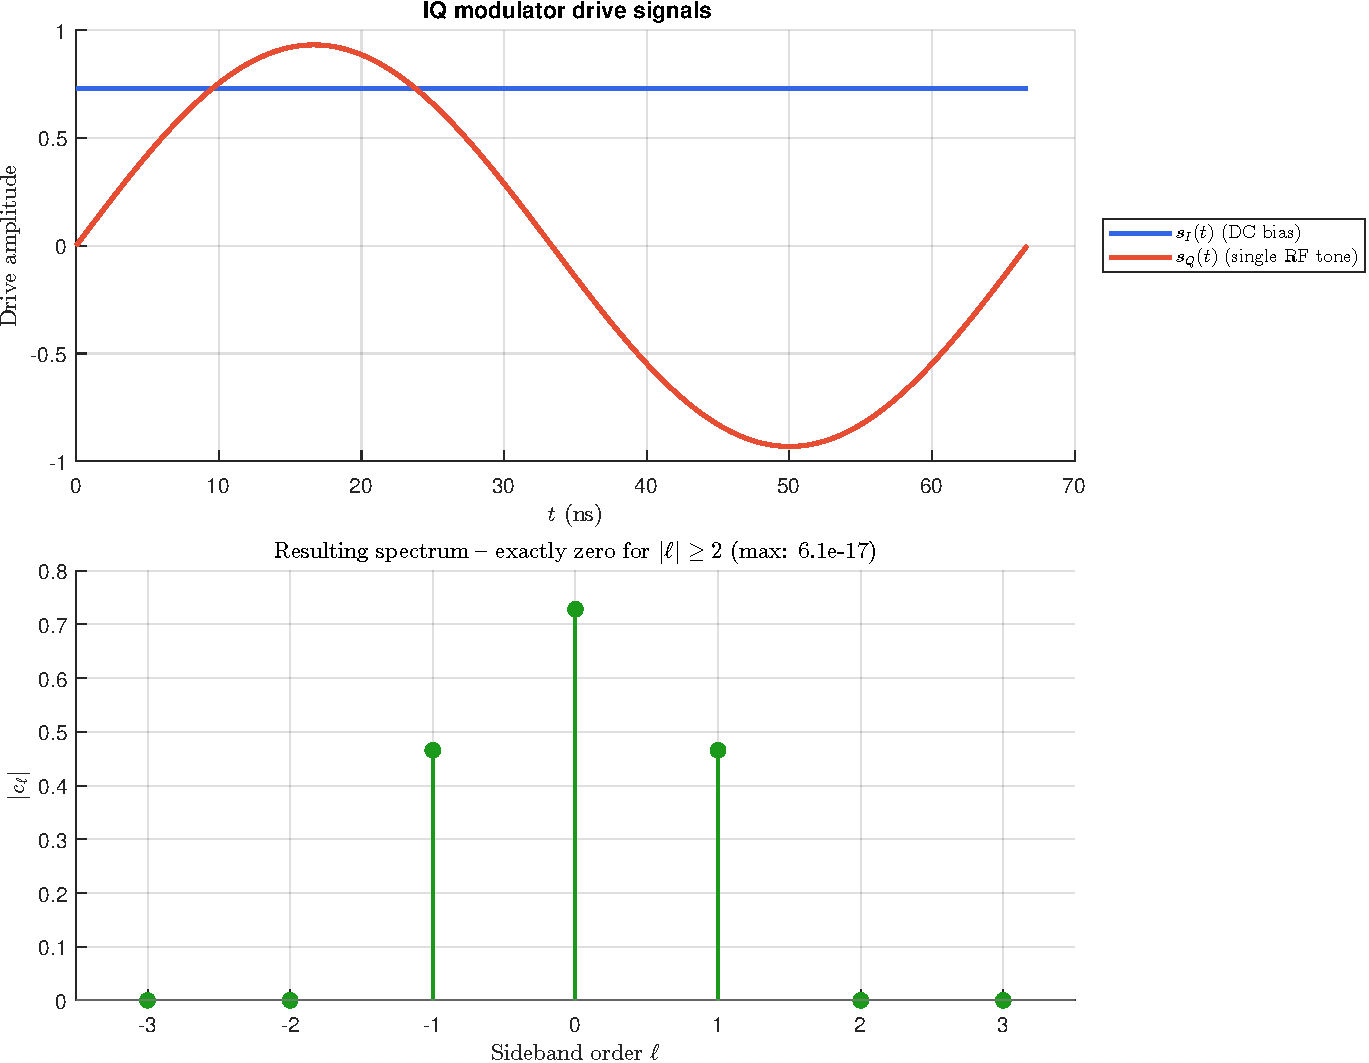
\includegraphics[width=0.75\textwidth]{pic/iq-modulator-spectrum.pdf}
\caption{Top: the IQ modulator drive signals $s_I(t)$, $s_Q(t)$
(\textit{generateIqModulatorDrive.m}) at
$\beta=$~Optimal~Modulation~Depth, $f_m=\SI{15}{\mega\hertz}$ --- a DC bias
and a single RF tone. Bottom: the resulting spectrum, recovered by an
FFT over one modulation cycle of the reconstructed envelope
$s_I(t)+i\,s_Q(t)$; exactly three lines, no higher orders, unlike
Figure~\ref{fig:sideband-regimes}'s EOM spectrum at the same $\beta$.}
\label{fig:iq-modulator-spectrum}
\end{figure}

\subsection{Where this leads}
\label{sec:sidebands-next}
Once the beam described by Eq.~\eqref{eq:pm-truncated} enters the cavity of
Section~\ref{sec:cavity}, each of its three frequency components sees its own
detuning from the nearest cavity resonance (Eq.~\eqref{eq:detuning-def}) ---
$\Delta f_{\mathrm{detune}}$ for the carrier, $\Delta f_{\mathrm{detune}} + f_m$
and $\Delta f_{\mathrm{detune}} - f_m$ for the upper and lower sideband --- and
so picks up its own value of the cavity's reflection coefficient
(Eq.~\eqref{eq:reflection}). If $f_m$ is far outside the cavity linewidth, the
two sidebands return
essentially untouched while the carrier alone is distorted near resonance.
Extracting that distortion --- the photodiode/mixer/filter detection chain,
and the phasor dot-product shortcut that reproduces it without simulating
time at all --- is the subject of the next sections of this report, to be
added as the corresponding tickets of the underlying wayfinder map are
worked through.

\section{The PDH Detection Chain}
\label{sec:pdh-detection}
\subsection{The full locking setup}
\label{sec:pdh-setup}
Section~\ref{sec:sidebands-next} left off with a beam --- carrier plus two
sidebands, either from an EOM (\S\ref{sec:sidebands-derivation}) or an IQ
modulator (\S\ref{sec:sidebands-iq-modulator}) --- reflecting off the cavity
of Section~\ref{sec:cavity}, each of its three lines picking up its own
value of the cavity's reflection coefficient. This section extracts a
usable error signal from that reflected light: the photodiode, mixer, and
low-pass filter that turn an optical field back into a single number a
servo could act on.
\begin{figure}[H]
\centering
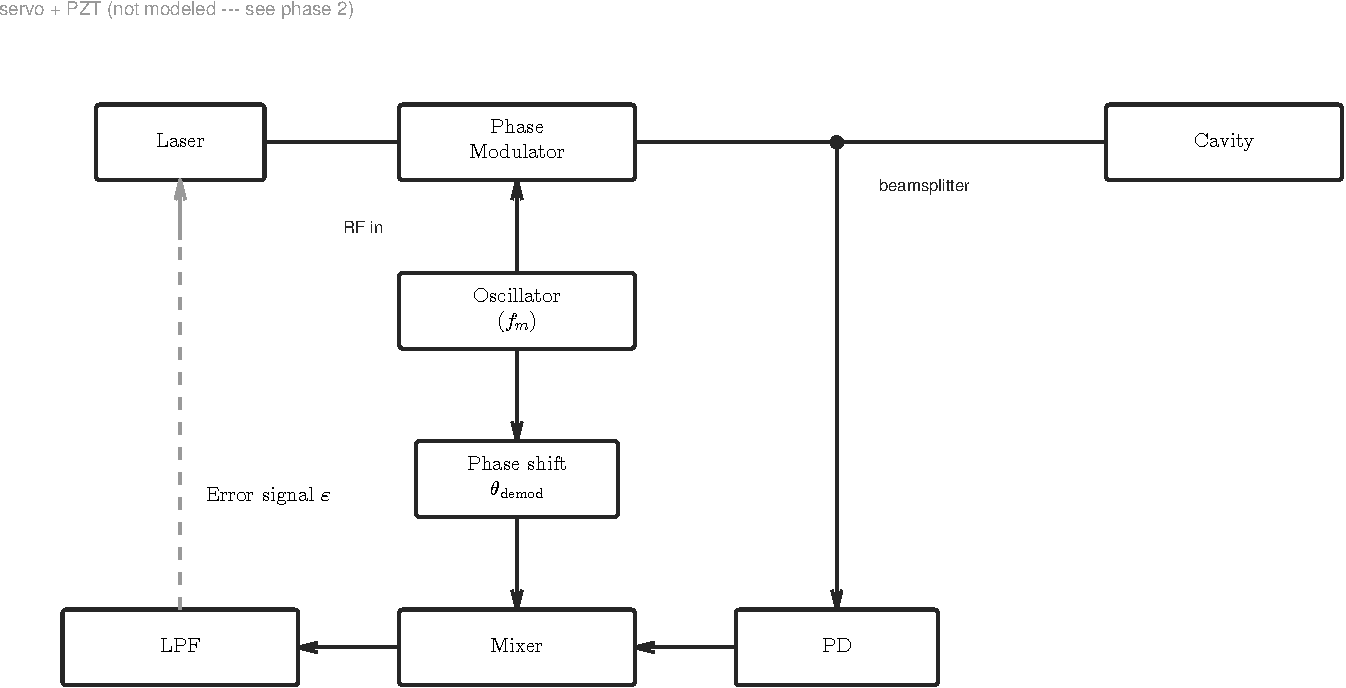
\includegraphics[width=\textwidth]{pic/pdh-detection-chain-schematic.pdf}
\caption{The full PDH laser-locking setup, schematically. The phase
modulator is drawn generically --- either \S\ref{sec:sidebands-derivation}'s
EOM or \S\ref{sec:sidebands-iq-modulator}'s IQ modulator can fill this role,
since nothing downstream depends on which one produced the sidebands. A
single oscillator at $f_m$ --- the local oscillator, or LO, in the mixer's
usual sense --- drives the modulator directly and, through an adjustable
phase shifter (the demodulation phase, named in
Section~\ref{sec:pdh-photodiode}), the mixer's other input. The servo and
PZT that would close the loop back onto the laser (grey, dashed) are not
modeled by this report --- see the ``Kick off phase-2 map'' ticket of the
underlying wayfinder map --- this section stops at the error signal
itself.}
\label{fig:pdh-detection-chain-schematic}
\end{figure}
Two things are worth naming before the math. First, the beamsplitter that
picks off the reflected beam for the photodiode is drawn as a plain,
generic element: this report has never modeled polarization, and a real
setup's polarizing-beamsplitter-plus-quarter-wave-plate isolation (keeping
reflected light out of the laser) would add a category of detail this
project doesn't otherwise track. Second, the single oscillator driving both
the modulator and (through its own phase shifter) the mixer is what makes
the demodulation phase meaningful at all: it is a phase \emph{relative to}
the modulation itself, not an absolute one, which is exactly why
Section~\ref{sec:pdh-demodulation} can tune it independently of everything
else in the chain.

\subsection{From reflected field to photodiode power}
\label{sec:pdh-photodiode}
Table~\ref{tab:pdh-glossary} collects the notation new to this section ---
everything else (\(J_\ell(\beta)\), \(r(\varphi)\), \(f_m\),
\(\Delta f_{\mathrm{detune}}\), \(\mathrm{FSR}\)) reuses Sections
\ref{sec:cavity} and \ref{sec:sidebands} exactly as already defined.
\begin{table}[H]
\centering
\small
\begin{tabular}{@{}llp{7cm}@{}}
\toprule
Symbol & Code identifier & Meaning \\
\midrule
$k$ & --- & harmonic-order label, $k\equiv\ell-\ell'\in\{-2,-1,0,1,2\}$, introduced by grouping Eq.~\eqref{eq:pdh-photodiode-power}'s terms --- distinct from Section~\ref{sec:cavity}'s round-trip index $k$ of Eqs.~\eqref{eq:transmission}--\eqref{eq:reflection} [forward-reference: that round-trip $k$ is a different, unrelated symbol that happens to share the letter, used earlier in the document; this table's own harmonic-order $k$ is not used before this point] \\
$\varphi_\ell$ & --- & per-line round-trip phase, extending Section~\ref{sec:cavity}'s $\varphi$ to each sideband's own detuning (Eq.~\eqref{eq:pdh-phi-ell}) \\
$\mathcal{E}_{\mathrm{refl},\ell}$ & --- & line $\ell$'s own reflected phasor, $\equiv \mathcal{E}_\ell\, r(\varphi_\ell)$ (Eq.~\eqref{eq:pdh-reflected-phasor}) --- extends \S\ref{sec:sidebands-phasors}'s phasor amplitude $\mathcal{E}_\ell$ through the cavity \\
$E_{\mathrm{refl}}(t)$ & --- & the cavity-reflected field's baseband envelope, carrier-frame (Eq.~\eqref{eq:pdh-reflected-field}) \\
$P_{\mathrm{PD}}(t)$ & --- & the photodiode's total power (Eq.~\eqref{eq:pdh-photodiode-power}) \\
$P_{\mathrm{PD,DC}}$ & \textit{dcReflectedPower} & the DC part of $P_{\mathrm{PD}}(t)$ (Eq.~\eqref{eq:pdh-pdc}) \\
$P_{\mathrm{PD},\omega_m}(t)$, $P_{\mathrm{PD},2\omega_m}(t)$ & \textit{computeReflectedPowerFrequencyScan} & its $\omega_m$/$2\omega_m$ parts (Eqs.~\eqref{eq:pdh-pd-omega-term}, \eqref{eq:pdh-pd-2omega-term}) \\
$C$ & --- & the beat-note coefficient at $\omega_m$ (Eq.~\eqref{eq:pdh-beat-coefficient}) \\
$D$ & --- & the beat-note coefficient at $2\omega_m$ (Eq.~\eqref{eq:pdh-2omega-coefficient}) \\
$\theta_{\mathrm{demod}}$ & \textit{DemodulationPhase} & the LO's own reference phase (Eq.~\eqref{eq:pdh-error-signal}) --- deliberately not bare $\theta$, to stay visually distinct from \S\ref{sec:sidebands-iq-modulator}'s unrelated $\theta_{\mathrm{IQ}}$ \\
$\varepsilon$ & \textit{errorSignal} & the demodulated PDH error signal (Eq.~\eqref{eq:pdh-error-signal}) \\
$\zeta$ & \textit{computePdh2OmegaSignalDotProduct} & the demodulated $2\omega_m$ signal (Eq.~\eqref{eq:pdh-zeta}) \\
\bottomrule
\end{tabular}
\caption{Notation used throughout Section~\ref{sec:pdh-detection}.}
\label{tab:pdh-glossary}
\end{table}
Each spectral line $\ell\in\{-1,0,1\}$ carries the cavity's own reflection
coefficient, evaluated at that line's own round-trip phase,
\begin{equation}
\varphi_\ell \equiv \frac{2\pi\left(\Delta f_{\mathrm{detune}} + \ell f_m\right)}{\mathrm{FSR}},
\label{eq:pdh-phi-ell}
\end{equation}
the same $\varphi=2\pi\Delta f_{\mathrm{detune}}/\mathrm{FSR}$ of
Eq.~\eqref{eq:detuning-def} (\S\ref{sec:cavity-derivation}), just evaluated
at $\Delta f_{\mathrm{detune}}+\ell f_m$ instead of $\Delta f_{\mathrm{detune}}$
alone --- $\varphi_0=\varphi$. Applying $r(\varphi_\ell)$ to line $\ell$'s
own phasor amplitude (\S\ref{sec:sidebands-phasors}'s $\mathcal{E}_\ell$)
gives that line's own reflected phasor,
\begin{equation}
\mathcal{E}_{\mathrm{refl},\ell} \equiv \mathcal{E}_\ell\, r(\varphi_\ell), \qquad \ell\in\{-1,0,1\},
\label{eq:pdh-reflected-phasor}
\end{equation}
so that recombining on the photodiode, the reflected field's baseband
envelope is
\begin{equation}
E_{\mathrm{refl}}(t) = \sum_{\ell=-1}^{1} \mathcal{E}_{\mathrm{refl},\ell}\, e^{i\ell\omega_m t},
\label{eq:pdh-reflected-field}
\end{equation}
Eq.~\eqref{eq:pm-truncated} with each line's own phasor now carried through
the cavity --- exactly the ``each frequency component picks up its own
value of the cavity's reflection coefficient'' of
\S\ref{sec:sidebands-next}, written out. A photodiode measures power, the
squared magnitude:
\begin{equation}
P_{\mathrm{PD}}(t) = \left|E_{\mathrm{refl}}(t)\right|^2 = \sum_{\ell=-1}^{1}\sum_{\ell'=-1}^{1} \mathcal{E}_{\mathrm{refl},\ell}\,\mathcal{E}_{\mathrm{refl},\ell'}^*\, e^{i(\ell-\ell')\omega_m t}.
\label{eq:pdh-photodiode-power}
\end{equation}
Grouping Eq.~\eqref{eq:pdh-photodiode-power}'s nine terms by
$k=\ell-\ell'\in\{-2,-1,0,1,2\}$ sorts them by frequency: the three $k=0$
terms carry no time dependence at all, the four $k=\pm1$ terms (two
distinct $(\ell,\ell')$ pairs each giving $k=+1$ and $k=-1$) oscillate at
$\omega_m$, and the two $k=\pm2$ terms oscillate at $2\omega_m$. Writing the
full split with each group its own named function of time,
\begin{equation}
P_{\mathrm{PD}}(t) = P_{\mathrm{PD,DC}} + P_{\mathrm{PD},\omega_m}(t) + P_{\mathrm{PD},2\omega_m}(t),
\label{eq:pdh-pd-split}
\end{equation}
we take each term in turn.

\paragraph{The DC term.} The three $k=0$ terms ($\ell=\ell'$) sum to
\begin{equation}
P_{\mathrm{PD,DC}} = \sum_{\ell=-1}^{1} \left|\mathcal{E}_{\mathrm{refl},\ell}\right|^2,
\label{eq:pdh-pdc}
\end{equation}
the incoherent sum of each line's own reflected power, obtained directly
without simulating any time domain at all (\textit{dcReflectedPower} in
\textit{simulatePdhErrorSignal.m} computes exactly this, bypassing
Eqs.~\eqref{eq:pdh-reflected-field}--\eqref{eq:pdh-photodiode-power}
entirely).

\paragraph{The $\omega_m$ term.} The four $k=\pm1$ terms are the two pairs
$(\ell,\ell')=(1,0)$ and $(0,-1)$:
\[
\mathcal{E}_{\mathrm{refl},1}\mathcal{E}_{\mathrm{refl},0}^*\,e^{i\omega_m t}
+ \mathcal{E}_{\mathrm{refl},0}\mathcal{E}_{\mathrm{refl},-1}^*\,e^{i\omega_m t}.
\]
Unlike the raw $J_\ell(\beta)$ products, these two terms need no further
sign-flip identity invoked here: $\mathcal{E}_{-1}=-\mathcal{E}_1$
(\S\ref{sec:sidebands-phasors}, itself inherited from
$J_{-1}(\beta)=-J_1(\beta)$) is already carried inside
$\mathcal{E}_{\mathrm{refl},-1}$, so the whole $e^{i\omega_m t}$ coefficient
is simply their sum, the beat-note coefficient
\begin{equation}
C \equiv \mathcal{E}_{\mathrm{refl},1}\mathcal{E}_{\mathrm{refl},0}^* + \mathcal{E}_{\mathrm{refl},0}\mathcal{E}_{\mathrm{refl},-1}^*,
\label{eq:pdh-beat-coefficient}
\end{equation}
% CHECKED-BY: ReportClaimsPdhTest.betaNoteCoefficientMatchesDirectHarmonicExtraction
giving
\begin{equation}
P_{\mathrm{PD},\omega_m}(t) \equiv Ce^{i\omega_m t}+C^*e^{-i\omega_m t} = 2\,\mathrm{Re}\!\left[Ce^{i\omega_m t}\right],
\label{eq:pdh-pd-omega-term}
\end{equation}
real as a physical power's piece must be, since the $k=+1$/$k=-1$ pair are
each other's complex conjugates (and, by the same token, so are the two
$k=\pm2$ terms making up $P_{\mathrm{PD},2\omega_m}(t)$ below). This is
the term \S\ref{sec:pdh-demodulation}'s mixer and low-pass filter extract
into the PDH error signal $\varepsilon$.

\paragraph{The $2\omega_m$ term.} The two $k=\pm2$ terms are the pair
$(\ell,\ell')=(1,-1)$:
\[
\mathcal{E}_{\mathrm{refl},1}\mathcal{E}_{\mathrm{refl},-1}^*\,e^{i2\omega_m t},
\]
already a single term --- the beat-note coefficient here is simply
\begin{equation}
D \equiv \mathcal{E}_{\mathrm{refl},1}\mathcal{E}_{\mathrm{refl},-1}^*,
\label{eq:pdh-2omega-coefficient}
\end{equation}
giving
\begin{equation}
P_{\mathrm{PD},2\omega_m}(t) \equiv De^{i2\omega_m t}+D^*e^{-i2\omega_m t} = 2\,\mathrm{Re}\!\left[De^{i2\omega_m t}\right],
\label{eq:pdh-pd-2omega-term}
\end{equation}
real as a physical power's piece must be, since the two $k=\pm2$ terms are
each other's complex conjugates. This is the term \S\ref{sec:pdh-demodulation}'s
doubled-LO mixer and its own low-pass filter extract into the demodulated
$2\omega_m$ signal $\zeta$. Unlike $C$, $D$
never involves $\varphi_0$ at all --- it depends only on the two
sidebands' own reflection coefficients, a fact
Figure~\ref{fig:pdh-photodiode-power-scan} below puts to direct use.
% CHECKED-BY: ReportClaimsPdhTest.photodiodePowerHasExactlyFiveHarmonics

\begin{figure}[H]
\centering
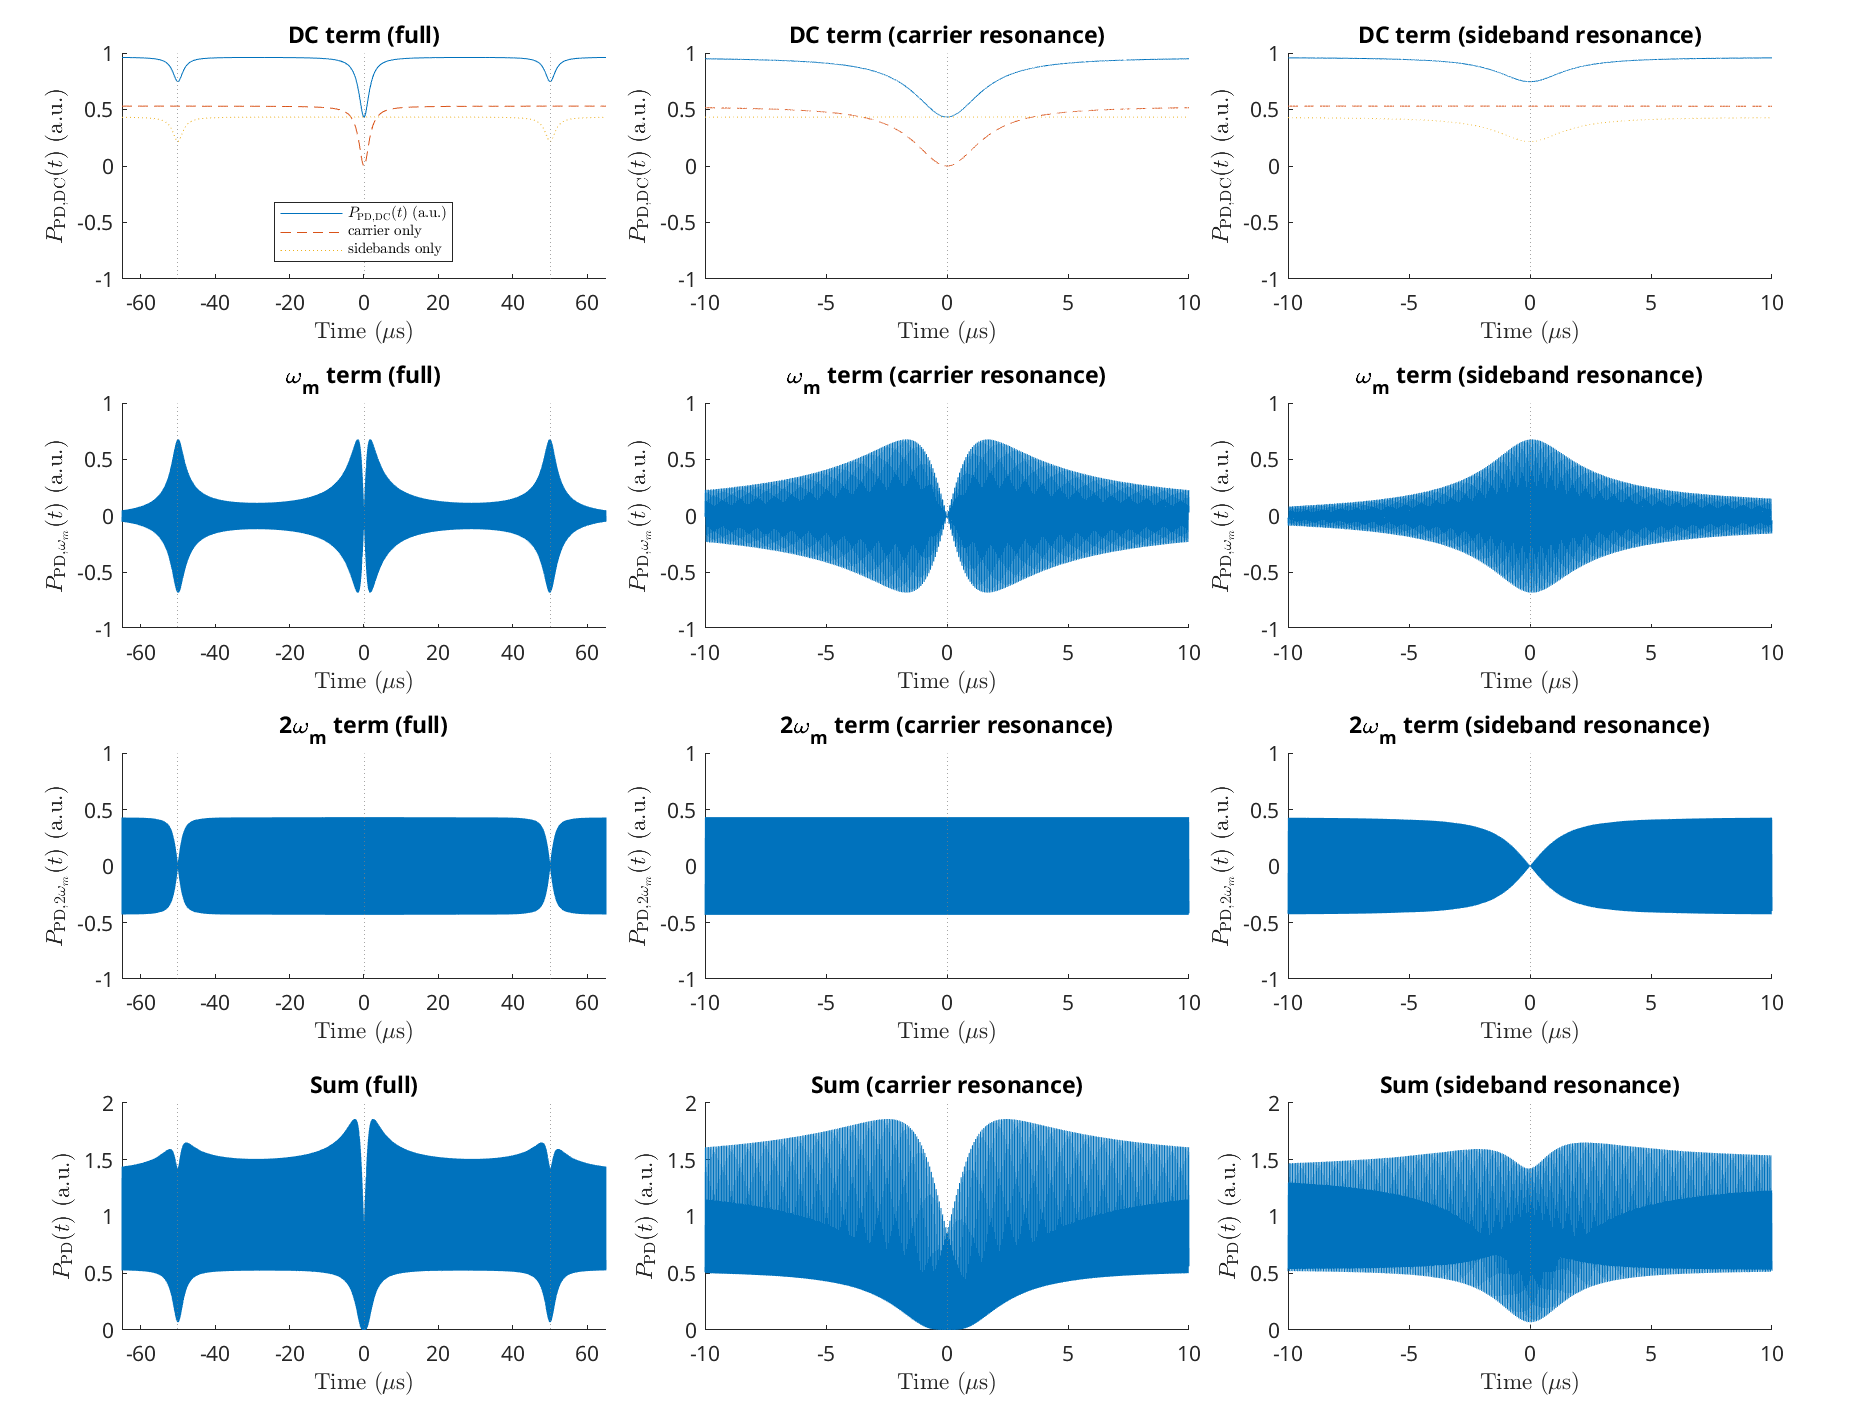
\includegraphics[width=\textwidth]{pic/pdh-photodiode-power-scan.pdf}
\caption{$P_{\mathrm{PD,DC}}(t)$, $P_{\mathrm{PD},\omega_m}(t)$,
$P_{\mathrm{PD},2\omega_m}(t)$, and their sum, over three matched windows
(Figure~\ref{fig:pdh-demodulated-signals} shares them), all on $[-1,1]$
except the sum (point 5): a full $\pm1.3f_m$ overview crossing all three
resonances, and a closer time-domain view ($\pm3$ linewidths) around the
carrier resonance and the representative sideband resonance at
$\Delta f_{\mathrm{detune}}=-f_m$ ($+f_m$ mirrors it) --- at this width
the fast oscillation is no longer individually resolved, only its
envelope. Time is referenced to $t=0$ at each column's own resonance;
dotted lines mark every resonance visible within a column. (1)
$P_{\mathrm{PD,DC}}(t)$ dips but never reaches zero: only the carrier's
own reflection nulls at critical coupling (dashed ``carrier only''); the
sidebands, $f_m$ away, keep reflecting almost fully (dotted ``sidebands
only''), setting the dip's floor. (2) In the carrier-resonance column,
$P_{\mathrm{PD},\omega_m}(t)$'s envelope pinches to a node and re-emerges
inverted right at resonance --- the zero-crossing
Figure~\ref{fig:pdh-demodulated-signals} shows already demodulated into
$\varepsilon$. (3) $P_{\mathrm{PD},2\omega_m}(t)$'s envelope is
essentially constant there, since $D$
(Eq.~\eqref{eq:pdh-2omega-coefficient}) depends only on the sidebands'
reflection coefficients, barely moved by this scan. (4) The
sideband-resonance column breaks that constancy: that sideband's own
field nulls, killing $D$ completely, while $C$ only loses one summand and
survives --- $P_{\mathrm{PD},\omega_m}(t)$ shows a same-signed bump
instead of a clean sign-flip; the carrier resonance alone kills the
$\omega_m$ term. (5) The sum exceeds $1$ even though each line
individually reflects and transmits without loss (\S\ref{sec:cavity-derivation}):
only the \emph{time-averaged} reflected+transmitted power matches the
time-averaged input (both below
$1$, \S\ref{sec:sidebands-derivation}) --- the cavity's frequency-dependent
response redistributes power \emph{in time} between the coherent lines,
like dispersion reshaping a pulse, not energy creation.}
\label{fig:pdh-photodiode-power-scan}
\end{figure}

\subsection{Demodulation}
\label{sec:pdh-demodulation}
For the PDH signal, the goal is to isolate the \emph{amplitude} of
$P_{\mathrm{PD}}(t)$'s $\omega_m$ component, $P_{\mathrm{PD},\omega_m}(t)$
(Eq.~\eqref{eq:pdh-pd-omega-term}), while preserving its \emph{phase} ---
that sign is exactly what tells a servo which side of resonance the laser
sits on. The way to do this is downmixing: multiply $P_{\mathrm{PD}}(t)$
by a reference signal at $\omega_m$ (the LO) and recover the amplitude by
low-pass filtering the result down to its own DC component.

\paragraph{The mixer.} The mixer multiplies $P_{\mathrm{PD}}(t)$ by the LO,
\[
\cos(\omega_m t+\theta_{\mathrm{demod}})=\tfrac12\left[e^{i(\omega_m t+\theta_{\mathrm{demod}})}+e^{-i(\omega_m t+\theta_{\mathrm{demod}})}\right],
\]
so every resulting cross-term sits at $0$, $\pm\omega_m$, or $\pm2\omega_m$ ---
never in between --- and the low-pass filter below keeps only the first:
the pair built from $C$, the $\omega_m$ beat-note coefficient already
derived in \S\ref{sec:pdh-photodiode} (Eq.~\eqref{eq:pdh-beat-coefficient}).

The same trick extracts the $2\omega_m$ terms too, one harmonic up: mixing
$P_{\mathrm{PD}}(t)$ against a frequency-doubled LO,
\[
\cos(2\omega_m t+2\theta_{\mathrm{demod}}) = \tfrac12\left[e^{i(2\omega_m t+2\theta_{\mathrm{demod}})}+e^{-i(2\omega_m t+2\theta_{\mathrm{demod}})}\right],
\]
isolates $D$'s $k=\pm2$ terms (Eq.~\eqref{eq:pdh-2omega-coefficient}),
making up $P_{\mathrm{PD},2\omega_m}(t)$, exactly as the $\omega_m$ LO
isolated $C$'s above. The reference phase doubles along with the
frequency because a real frequency doubler derives this second LO from
the very same oscillator driving the $\omega_m$ mixer: squaring
$\cos(\omega_m t+\theta_{\mathrm{demod}})$ produces a $2\omega_m$ term with
phase $2\theta_{\mathrm{demod}}$, not a second, independently adjustable
phase. This second channel --- $D$, the same coefficient defined in
\S\ref{sec:pdh-photodiode} (Eq.~\eqref{eq:pdh-2omega-coefficient}) --- is
carried through its own low-pass filter alongside $\varepsilon$ below, the
same way.

\paragraph{The low-pass filter.} Exactly two of the mixer's cross-terms land at zero frequency: pairing
$Ce^{i\omega_m t}$ with the LO's $e^{-i(\omega_m t+\theta_{\mathrm{demod}})}$
half gives $\tfrac12 Ce^{-i\theta_{\mathrm{demod}}}$, and pairing
$C^*e^{-i\omega_m t}$ with $e^{i(\omega_m t+\theta_{\mathrm{demod}})}$
gives its own complex conjugate, $\tfrac12C^*e^{i\theta_{\mathrm{demod}}}$.
Every other cross-term --- $P_{\mathrm{PD,DC}}\cos(\omega_m t+\theta_{\mathrm{demod}})$
itself, and the $k=\pm2$ terms against the LO --- sits at $\pm\omega_m$ or
$\pm2\omega_m$ and is removed by the low-pass filter
(\textit{simulatePdhErrorSignal.m} designs a 4th-order IIR filter at
one-tenth of $f_m$, applied zero-phase via \texttt{filtfilt}). What survives
is real by construction, a sum of conjugates:
\begin{equation}
\varepsilon\!\left(\Delta f_{\mathrm{detune}}\right) \equiv \tfrac12\left[Ce^{-i\theta_{\mathrm{demod}}} + C^*e^{i\theta_{\mathrm{demod}}}\right] = \mathrm{Re}\!\left[C\,e^{-i\theta_{\mathrm{demod}}}\right],
\label{eq:pdh-error-signal}
\end{equation}
the PDH error signal --- exactly what \textit{simulatePdhErrorSignal.m}
returns, verified there against this same closed form to within numerical
noise, cross-checked independently of its own time-domain simulation.
% CHECKED-BY: ReportClaimsPdhTest.errorSignalMatchesClosedForm

The doubled-LO channel above survives the same way.
Pairing $De^{i2\omega_m t}$ with that LO's $e^{-i(2\omega_m t+2\theta_{\mathrm{demod}})}$
half gives $\tfrac12 De^{-i2\theta_{\mathrm{demod}}}$, its conjugate pairing
gives $\tfrac12D^*e^{i2\theta_{\mathrm{demod}}}$, and every other
cross-term is removed by that channel's own low-pass filter, leaving
\begin{equation}
\zeta\!\left(\Delta f_{\mathrm{detune}}\right) \equiv \tfrac12\left[De^{-i2\theta_{\mathrm{demod}}} + D^*e^{i2\theta_{\mathrm{demod}}}\right] = \mathrm{Re}\!\left[D\,e^{-i2\theta_{\mathrm{demod}}}\right],
\label{eq:pdh-zeta}
\end{equation}
the demodulated $2\omega_m$ signal --- \textit{computePdh2OmegaSignalDotProduct.m}
computes exactly this closed form directly; no time-domain simulation of
this second channel exists in this project, mirroring the closed-form
shortcut \S\ref{sec:pdh-next} previews for $\varepsilon$ itself. Unlike
$\varepsilon$, which is odd in $\Delta f_{\mathrm{detune}}$
(Eq.~\eqref{eq:pdh-error-signal}'s S-curve), $\zeta$ is \emph{even}: $D$
pairs $r(\Delta f_{\mathrm{detune}}+f_m)$ with
$r^*(\Delta f_{\mathrm{detune}}-f_m)$, and
$r(-\varphi)=r^*(\varphi)$ (immediate from Eq.~\eqref{eq:reflection},
since $r_1,r_2$ are both real) makes that product symmetric under
$\Delta f_{\mathrm{detune}}\to-\Delta f_{\mathrm{detune}}$. $\zeta$ also
vanishes exactly at each sideband resonance
($\Delta f_{\mathrm{detune}}=\mp f_m$, where that sideband's own field
nulls and kills $D$ outright, \S\ref{sec:pdh-photodiode}) but --- unlike
$\varepsilon$ --- does \emph{not} null at the carrier resonance
($\Delta f_{\mathrm{detune}}=0$), since $D$ never involves $\varphi_0$ at
all.

Eq.~\eqref{eq:pdh-error-signal} also shows concretely why the demodulation
phase in \S\ref{sec:sidebands-motivation}'s ``mixing down'' step is a real
design choice, not a formality: $\theta_{\mathrm{demod}}$ rotates $C$
before taking its real part, and $C$'s own phase need not point the same
way at every detuning. At
$\Delta f_{\mathrm{detune}}=0.5\,\Delta\nu_{\mathrm{FWHM}}$ (this project's
running example, $\beta\approx1.08$), $\varepsilon=0.339$ at
$\theta_{\mathrm{demod}}=\pi/2$ but only $\varepsilon=0.0113$ at
$\theta_{\mathrm{demod}}=0$ --- almost $30\times$ smaller, not merely
scaled down --- while at
$\Delta f_{\mathrm{detune}}=f_m+0.5\,\Delta\nu_{\mathrm{FWHM}}$ (the
secondary, sideband-resonance feature Figure~\ref{fig:pdh-demodulated-signals}'s
sideband-resonance column shows), the two phases swap roles: $\theta_{\mathrm{demod}}=0$
gives the larger signal there. The carrier-locking feature this section
exists to produce and the sideband-resonance feature live in orthogonal
demodulation quadratures, which is why this project's default is
$\theta_{\mathrm{demod}}=\pi/2$, not $0$.
% CHECKED-BY: ReportClaimsPdhTest.demodulationPhaseSuppressesCarrierFeatureByThirtyFold

Figure~\ref{fig:pdh-demodulated-signals} revisits the exact three windows
Figure~\ref{fig:pdh-photodiode-power-scan} used in the time domain, now
already demodulated: $P_{\mathrm{PD,DC}}$, $\varepsilon$, and $\zeta$ over
the identical detuning ranges, so the two figures can be read side by side
without their windows ever silently drifting apart. The carrier-resonance
column is the same clean, sign-flipping zero-crossing
Figure~\ref{fig:pdh-photodiode-power-scan} showed as a raw envelope pinch
in $P_{\mathrm{PD},\omega_m}(t)$; the sideband-resonance column is the
smaller, same-signed bump that same term showed there too, now easy to
read off directly as a curve. $\zeta$'s own row makes
Eq.~\eqref{eq:pdh-zeta}'s even symmetry and its exact sideband-resonance
null immediately visible, mirroring $P_{\mathrm{PD},2\omega_m}(t)$'s
envelope in the time domain.
\begin{figure}[H]
\centering
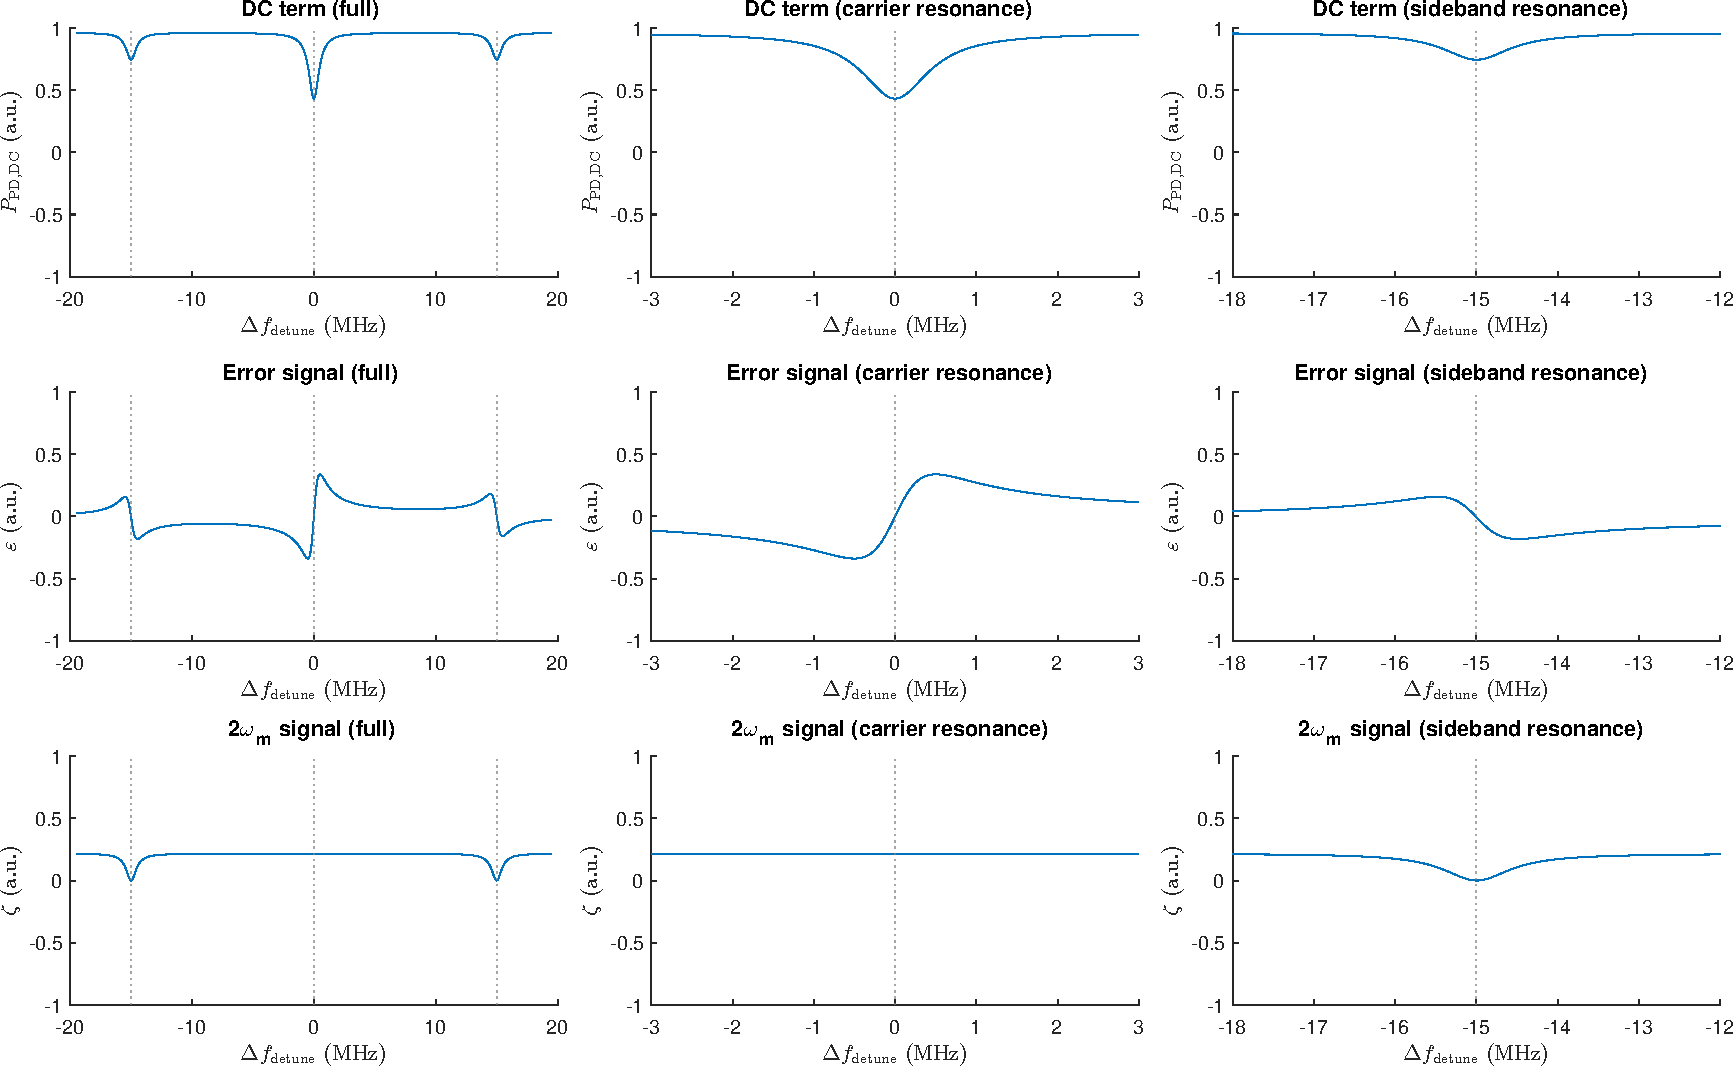
\includegraphics[width=0.85\textwidth]{pic/pdh-demodulated-signals-spans.pdf}
\caption{$P_{\mathrm{PD,DC}}$, the demodulated error signal $\varepsilon$,
and its $2\omega_m$ counterpart $\zeta$ (Eq.~\eqref{eq:pdh-zeta}) vs.\
detuning, over the exact same three windows (full, carrier resonance,
sideband resonance) as Figure~\ref{fig:pdh-photodiode-power-scan}'s
time-domain view, all on the same $[-1,1]$ vertical scale --- both figures
read the same underlying spans (\textit{pdhPhotodiodeScanSpans.m}), so
they cannot drift out of sync with each other. The carrier-resonance
column is the dispersive S-curve of Eq.~\eqref{eq:pdh-error-signal} ---
$\zeta$ shows no feature there at all, since $D$ never involves $\varphi_0$;
the sideband-resonance column is $\varepsilon$'s secondary feature from the
$\theta_{\mathrm{demod}}$ discussion above, together with $\zeta$'s exact
null there.}
\label{fig:pdh-demodulated-signals}
\end{figure}

\subsection{Where this leads}
\label{sec:pdh-next}
Eq.~\eqref{eq:pdh-error-signal} was reached by simulating a photodiode, a
mixer, and a filter numerically --- exactly what
\textit{simulatePdhErrorSignal.m} does, sample by sample, at every
detuning. None of that simulation was actually necessary: $C$
(Eq.~\eqref{eq:pdh-beat-coefficient}) is built entirely from the three
lines' own reflected fields, with no time dependence left in it at all, and
$\varepsilon=\mathrm{Re}(Ce^{-i\theta_{\mathrm{demod}}})$ is nothing more
than a fixed rotation of a fixed complex number. Section~\ref{sec:pdh-dotproduct}
makes that explicit: it shows $C$ is a phasor dot product between the
carrier's own reflected field and a combination of the two sidebands' ---
the same $\varepsilon$, reached without ever constructing $E_{\mathrm{refl}}(t)$,
$P_{\mathrm{PD}}(t)$, or a single time sample.

\section{The Phasor Dot-Product Shortcut}
\label{sec:pdh-dotproduct}
\subsection{The dot-product identity}
\label{sec:pdh-dotproduct-derivation}
Table~\ref{tab:pdh-dotproduct-glossary} collects the one symbol new to this
section; everything else ($\mathcal{E}_\ell$, $\mathcal{E}_{\mathrm{refl},\ell}$,
$\theta_{\mathrm{demod}}$, $C$, $\varepsilon$) reuses
Sections~\ref{sec:sidebands} and \ref{sec:pdh-detection} exactly as already
defined.
\begin{table}[H]
\centering
\small
\begin{tabular}{@{}llp{7cm}@{}}
\toprule
Symbol & Code identifier & Meaning \\
\midrule
$\mathcal{E}_{\mathrm{refl,sb}}$ & --- & the sideband resultant phasor, the two sidebands' own reflected phasors combined at the demodulation phase (Eq.~\eqref{eq:pdh-dotproduct-sideband-resultant}) \\
\bottomrule
\end{tabular}
\caption{Notation used throughout Section~\ref{sec:pdh-dotproduct}.}
\label{tab:pdh-dotproduct-glossary}
\end{table}
For any two complex numbers $z,w$, treating each as a real 2D vector
$(\mathrm{Re},\mathrm{Im})$ makes an otherwise-opaque piece of complex
algebra literal:
\begin{equation}
\mathrm{Re}(z\,w^*) = \mathrm{Re}(z)\,\mathrm{Re}(w) + \mathrm{Im}(z)\,\mathrm{Im}(w) \equiv z\cdot w = |z|\,|w|\cos(\phi_z-\phi_w),
\label{eq:pdh-dotproduct-lemma}
\end{equation}
the ordinary real dot product of the two vectors --- exactly
\textit{PhasorMath.dotProduct}, and, via the cosine form (writing
$z=|z|e^{i\phi_z}$, $w=|w|e^{i\phi_w}$), the length of $w$'s projection onto
$z$'s own direction, scaled by $|z|$: it is maximized when the two phasors
point the same way ($\phi_z=\phi_w$), zero when they are perpendicular, and
flips sign once they point more than $90^\circ$ apart. Section~\ref{sec:pdh-photodiode} already
built the beat-note coefficient
$C=\mathcal{E}_{\mathrm{refl},1}\mathcal{E}_{\mathrm{refl},0}^*+\mathcal{E}_{\mathrm{refl},0}\mathcal{E}_{\mathrm{refl},-1}^*$
(Eq.~\eqref{eq:pdh-beat-coefficient}) and the error signal
$\varepsilon=\mathrm{Re}[Ce^{-i\theta_{\mathrm{demod}}}]$
(Eq.~\eqref{eq:pdh-error-signal}) out of it --- a sum in which the
carrier's own reflected phasor $\mathcal{E}_{\mathrm{refl},0}$ appears,
once conjugated and once not, multiplying each sideband's reflected
phasor in turn. Substituting $C$ into $\varepsilon$ and using
$\mathrm{Re}(u^*)=\mathrm{Re}(u)$ on the $\mathcal{E}_{\mathrm{refl},1}$
term (to flip which factor carries the conjugate without changing the real
part it contributes) lets the shared factor $\mathcal{E}_{\mathrm{refl},0}$
be pulled out from under a single, common conjugate:
\begin{equation}
\varepsilon = \mathrm{Re}\!\left[\mathcal{E}_{\mathrm{refl},0}\,\left(\mathcal{E}_{\mathrm{refl},1}e^{-i\theta_{\mathrm{demod}}} + \mathcal{E}_{\mathrm{refl},-1}e^{i\theta_{\mathrm{demod}}}\right)^*\right].
\label{eq:pdh-dotproduct-rearrangement}
\end{equation}
% CHECKED-BY: ReportClaimsDotProductTest.rearrangementMatchesOriginalErrorSignal
Naming the parenthesized sum
\begin{equation}
\mathcal{E}_{\mathrm{refl,sb}} \equiv \mathcal{E}_{\mathrm{refl},1}e^{-i\theta_{\mathrm{demod}}} + \mathcal{E}_{\mathrm{refl},-1}e^{i\theta_{\mathrm{demod}}}
\label{eq:pdh-dotproduct-sideband-resultant}
\end{equation}
--- the two sidebands' own reflected phasors, each rotated by the
demodulation phase in opposite directions (since they counter-rotate,
\S\ref{sec:sidebands-phasors}) and summed --- turns
Eq.~\eqref{eq:pdh-dotproduct-rearrangement} into exactly
Eq.~\eqref{eq:pdh-dotproduct-lemma}'s dot product:
\begin{equation}
\varepsilon = \mathrm{Re}\!\left[\mathcal{E}_{\mathrm{refl},0}\,\mathcal{E}_{\mathrm{refl,sb}}^*\right] = \mathcal{E}_{\mathrm{refl},0}\cdot\mathcal{E}_{\mathrm{refl,sb}}.
\label{eq:pdh-dotproduct-identity}
\end{equation}
% CHECKED-BY: ReportClaimsDotProductTest.dotProductIdentityMatchesOriginalErrorSignal
This is the promise \S\ref{sec:pdh-next} closed on: the same error signal
already derived in \S\ref{sec:pdh-demodulation}, understood geometrically,
is the dot product of the carrier's own reflected phasor with the
(demodulation-phase-combined) sideband resultant --- two fixed complex
numbers at any given detuning.

\paragraph{What the demodulation phase actually controls.}
$\mathcal{E}_{\mathrm{refl},1}e^{-i\theta_{\mathrm{demod}}}$ and
$\mathcal{E}_{\mathrm{refl},-1}e^{i\theta_{\mathrm{demod}}}$ each rotate
rigidly, oppositely, as $\theta_{\mathrm{demod}}$ sweeps --- but their sum
$\mathcal{E}_{\mathrm{refl,sb}}$ generally does not: two counter-rotating
phasors of unequal magnitude trace an ellipse, not a circle, as
$\theta_{\mathrm{demod}}$ completes a turn. That ellipse degenerates to a
rigid rotation only where one term vanishes outright ---
\S\ref{sec:pdh-resonance-case-walkthrough}'s side-mode-resonance case is
exactly this: the upper term is zero there, so
$\mathcal{E}_{\mathrm{refl,sb}}(\theta_{\mathrm{demod}}) = \mathcal{E}_{\mathrm{refl},-1}e^{i\theta_{\mathrm{demod}}}$
alone, and it does rotate rigidly, verified to floating-point precision.
Away from such a point the resultant's own path is generally more
complicated than either a rotation or a fixed direction, so nothing about
$I$ and $Q$ being orthogonal can be read off its motion in general.
% CHECKED-BY: ReportClaimsDotProductTest.sidebandResultantRotatesRigidlyOnlyWhenOneTermVanishes
What \emph{is} always true, with no such caveat, is a direct consequence of
Eq.~\eqref{eq:pdh-error-signal}: $\varepsilon(\theta_{\mathrm{demod}})=\mathrm{Re}[Ce^{-i\theta_{\mathrm{demod}}}]$
is a pure cosine in $\theta_{\mathrm{demod}}$, of amplitude $|C|$ and phase
offset $\arg C$, regardless of how $\mathcal{E}_{\mathrm{refl,sb}}$ itself
moves --- Eq.~\eqref{eq:pdh-dotproduct-identity} identifies this cosine as
$\mathcal{E}_{\mathrm{refl},0}$ dotted against
$\mathcal{E}_{\mathrm{refl,sb}}(\theta_{\mathrm{demod}})$. Reading
$\theta_{\mathrm{demod}}=0$ and $\theta_{\mathrm{demod}}=\pi/2$ off that one
cosine gives exactly $\mathrm{Re}(C)$ and $\mathrm{Im}(C)$: Q and I are the
real and imaginary parts of the single complex number this section's dot
product already computes, which is why they are orthogonal --- in the
ordinary sense that real and imaginary parts are --- without either
sideband resultant needing to visibly rotate through $90^\circ$ to make
them so. This is exactly \textit{computePdhErrorSignalDotProduct.m}
(\textit{PhasorMath.dotProduct} applied to
\textit{PhasorMath.sidebandAmplitude} and
\textit{PhasorMath.combineAtDemodulationPhase}'s outputs), already
cross-checked against \S\ref{sec:pdh-demodulation}'s time-domain
$\varepsilon$ to within numerical noise.
% CHECKED-BY: ReportClaimsDotProductTest.errorSignalIsPureCosineGivingRealAndImaginaryPartsOfC

\subsection{A detuning-by-detuning walkthrough}
\label{sec:pdh-resonance-case-walkthrough}
A single representative snapshot of Eq.~\eqref{eq:pdh-dotproduct-identity}'s
phasor picture is not enough to see \emph{why} the dot product takes the
values it does as detuning actually sweeps through the cavity's resonance
structure. Figure~\ref{fig:pdh-resonance-case-walkthrough} below evaluates
the PDH cavity at four characteristic detunings, one row each, showing all
four faces of the picture together: (a) the phasor diagram --- carrier
phasor (green), the two sideband phasors combined into the sideband
resultant (blue/red arrows and their black sum), and the dot product
between them (shaded projection) --- fixed to a common $[-1,1]$ scale so
magnitude changes between rows are directly comparable rather than hidden
by auto-scaling; (b) the resulting
PDH error signal $\varepsilon(\Delta f)$ of
Eq.~\eqref{eq:pdh-dotproduct-identity}, marked at that row's own detuning;
(c) the reflected power $|r(\Delta f)|^2$; and (d) the reflected phase
$\arg r(\Delta f)$, unwrapped --- the same construction
\textit{animatePdhDetuningScanPhasors.m}'s live tool draws, frozen at four
illustrative points instead of animated. All four rows share one background
detuning span (the same $1.3f_m$ span the live tool itself uses), and
panels (c)/(d) mark all three lines on that shared curve at once: the
carrier's own detuning (green), the upper sideband's (blue), and the lower
sideband's (red) --- three evaluations of the identical response function,
not three different curves.
\begin{figure}[H]
\centering
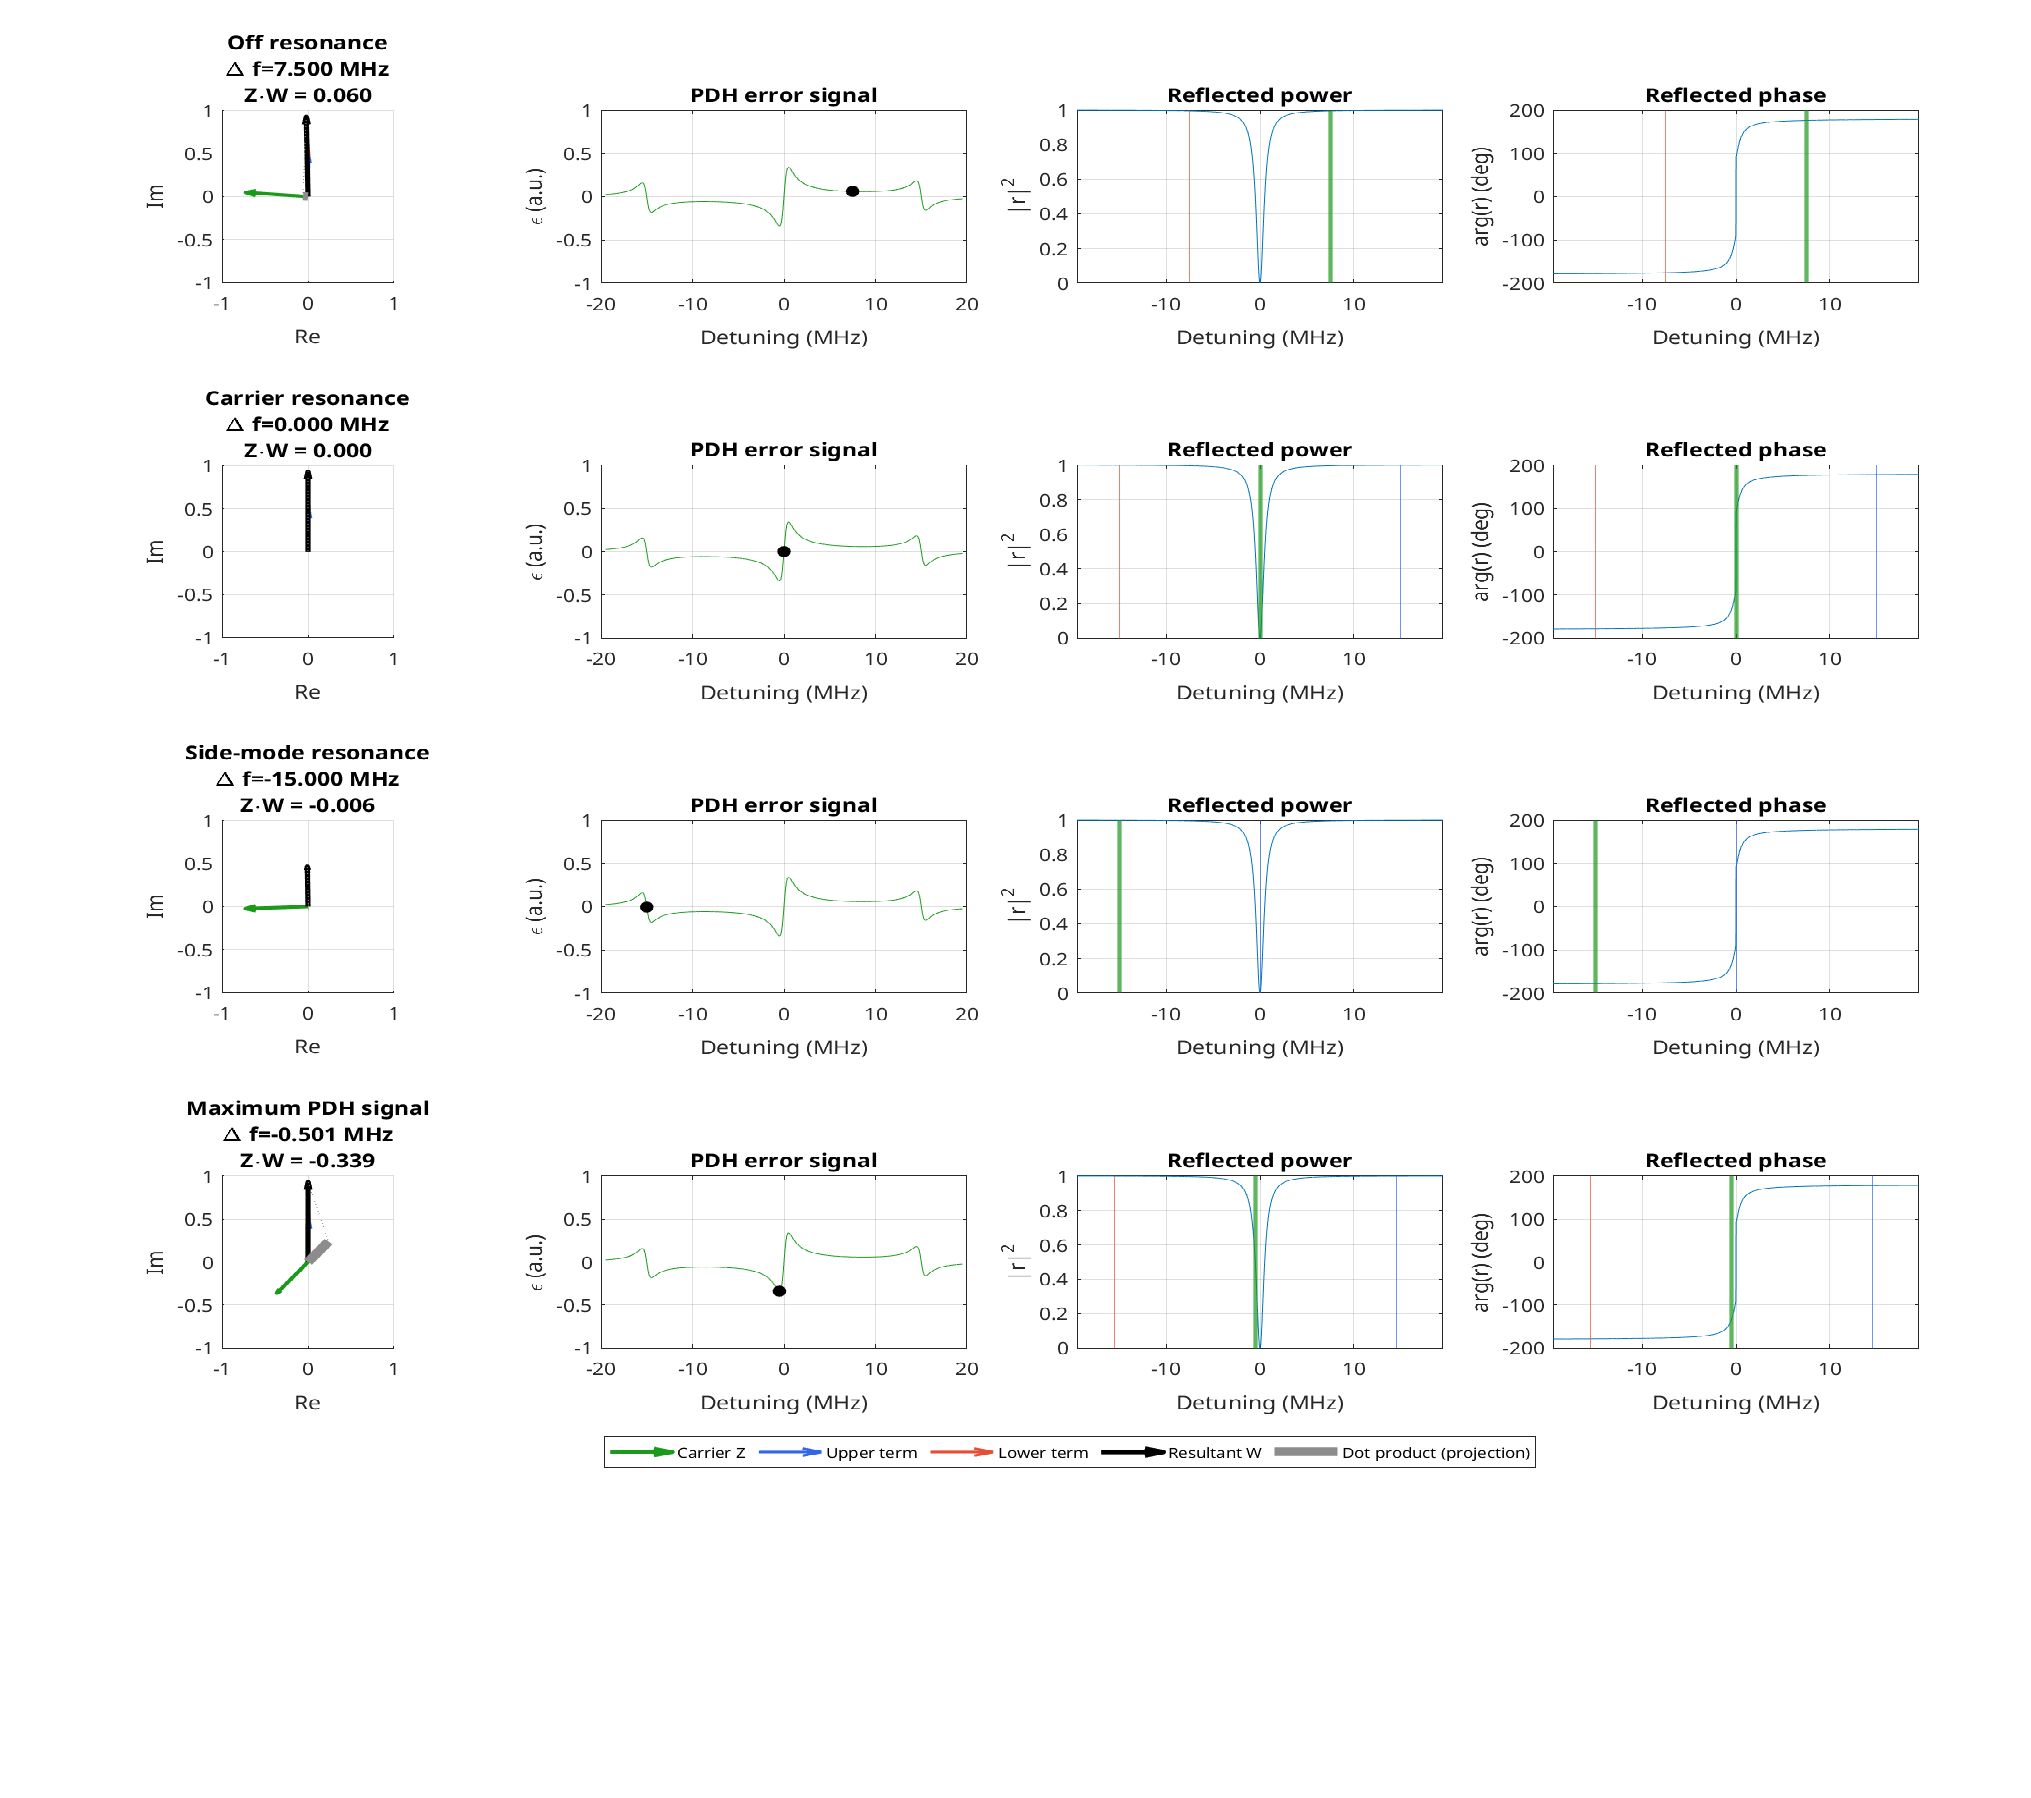
\includegraphics[width=\textwidth]{pic/pdh-resonance-case-walkthrough.pdf}
\caption{Four characteristic detunings of the PDH cavity example, one row
each: off resonance, carrier resonance, side-mode resonance, and the
detuning that numerically maximizes $|\varepsilon(\Delta f)|$. Column (a)
phasors on a common $[-1,1]$ scale; (b) the error signal with a marker at
the row's detuning; (c)/(d) reflected power/phase with markers at the
carrier's (green), upper sideband's (blue), and lower sideband's (red) own
detuning.}
\label{fig:pdh-resonance-case-walkthrough}
\end{figure}

\paragraph{Case 1: off resonance ($\Delta f=f_m/2$).} This detuning is
$7.5$ linewidths from the carrier's own resonance and, by construction,
equally $7.5$ linewidths from each sideband resonance at $\pm f_m$ --- the
most off-resonance point available inside the shared span. All three lines
therefore sit far enough into the background that their reflectivity is
nearly identical: $|r(\Delta f)|^2=0.996$, close to the mirror's own
asymptotic background, with $\arg r(\Delta f)=176.2^\circ$, just short of
the $180^\circ$ a truly infinite detuning would give --- $f_m$ is only $15$
linewidths from the carrier's resonance, not infinitely many, so a small
residual survives here deliberately rather than being rounded away.
Because all three lines share nearly the same phase,
$\mathcal{E}_{\mathrm{refl},0}\approx-0.725+0.048i$ sits almost exactly on
the negative real axis, and so does the raw upper-sideband term
$\mathcal{E}_{\mathrm{refl},1}\approx-0.465+0.010i$, while the raw lower
term is very nearly its negative,
$\mathcal{E}_{\mathrm{refl},-1}\approx-\mathcal{E}_{\mathrm{refl},1}$, from
$\mathcal{E}_{-1}=-\mathcal{E}_1$ (\S\ref{sec:sidebands-derivation}) acting
on two nearly-equal reflectivities. With
$\mathcal{E}_{\mathrm{refl},-1}=-\mathcal{E}_{\mathrm{refl},1}$,
Eq.~\eqref{eq:pdh-dotproduct-sideband-resultant} collapses to
\[
\mathcal{E}_{\mathrm{refl,sb}}(\theta_{\mathrm{demod}}) = \mathcal{E}_{\mathrm{refl},1}\left(e^{-i\theta_{\mathrm{demod}}}-e^{i\theta_{\mathrm{demod}}}\right) = -2i\,\mathcal{E}_{\mathrm{refl},1}\sin\theta_{\mathrm{demod}}
\]
--- $\mathcal{E}_{\mathrm{refl},1}$ rotated by exactly $90^\circ$, for every
$\theta_{\mathrm{demod}}$ and every modulation depth $\beta$ (exact to
floating-point precision with no cavity at all). The $90^\circ$ angle is
fixed by phase modulation's own sideband symmetry, not by any tunable
parameter of this system. The one thing that moves it away from $90^\circ$
is \textbf{detuning}: close enough to an actual resonance, the cavity stops
giving the carrier and the sidebands the same phase, and
$\arg\mathcal{E}_{\mathrm{refl},1}\ne\arg\mathcal{E}_{\mathrm{refl},0}$ ---
exactly the $84.9^\circ$, not $90^\circ$, measured here.
% CHECKED-BY: ReportClaimsDotProductTest.offResonancePerpendicularityIsIndependentOfDemodulationPhase
Two (nearly) perpendicular phasors dot to almost nothing: $\varepsilon=0.060$,
about $18\%$ of this cavity's peak (case 4 below) and the
smallest-magnitude of the four cases.

\paragraph{Case 2: carrier resonance ($\Delta f=0$).} The carrier itself
now sits exactly on resonance. Critical coupling makes $r(0)=0$ exactly
(\S\ref{sec:cavity-response}), so $\mathcal{E}_{\mathrm{refl},0}$ vanishes
outright --- panel (a) shows no carrier arrow at all. The sidebands, still
$f_m=15$ linewidths away, are essentially unmoved from case 1's own
background value ($\mathcal{E}_{\mathrm{refl,sb}}=0.930i$ here, purely
imaginary to three digits). The dot product of anything with the zero
vector is zero: $\varepsilon=0$ exactly, not approximately --- a different
mechanism from case 1's near-perpendicularity, even though both land at or
near zero.

\paragraph{Case 3: side-mode resonance ($\Delta f=-f_m$).} Detuning the
carrier by exactly one modulation frequency below its own resonance parks
the \emph{upper} sideband exactly on resonance instead
($\Delta f+f_m=0$), so its own reflected phasor vanishes: the upper term
drops out of $\mathcal{E}_{\mathrm{refl,sb}}$ entirely, leaving only the
lower term ($\mathcal{E}_{\mathrm{refl,sb}}=-0.008+0.466i$, half the
magnitude of case 1's fully-populated resultant). The carrier itself,
sitting $f_m=15$ linewidths from its own resonance, is still essentially at
background ($\mathcal{E}_{\mathrm{refl},0}=-0.727-0.024i$). Despite one
sideband dropping out, the dot product is still small
($\varepsilon=-0.006$): the carrier and the now-smaller resultant are still
close to perpendicular, for the same reason as case 1. It is not, however,
exactly zero the way case 2 is --- this secondary dispersive feature's true
zero-crossing sits a small fraction of a linewidth away from
$\Delta f=-f_m$, precisely because $f_m/\Delta\nu_{\mathrm{FWHM}}=15$ is
large but finite, not infinite.

\paragraph{Case 4: maximum PDH signal
($\Delta f=-0.501\,\Delta\nu_{\mathrm{FWHM}}$).} Found numerically as the
detuning that maximizes $|\varepsilon(\Delta f)|$ across the shared span
(the same search \S\ref{sec:pdh-demodulation} already used to establish
this cavity's own canonical point), this is where the carrier's own
dispersive feature --- not any sideband feature --- does the work. Here
$\mathcal{E}_{\mathrm{refl},0}=-0.365-0.364i$: its real and imaginary parts
are equal in magnitude to three significant figures, i.e.
$\arg(\mathcal{E}_{\mathrm{refl},0})=-135.1^\circ$, exactly $45^\circ$ away
from case 1's off-resonance background direction of
$\approx\!176$--$178^\circ$. This is the general extremum condition for a
complex, Lorentzian-like response: the component of
$\mathcal{E}_{\mathrm{refl},0}$ perpendicular to the background direction
--- the part a $\theta_{\mathrm{demod}}=\pi/2$ demodulation actually senses
--- is maximized exactly where the phasor has rotated a further $45^\circ$
from where it started. The sideband resultant is essentially unchanged from
every other case ($\mathcal{E}_{\mathrm{refl,sb}}=0.001+0.930i$, since
$\pm f_m$ is unaffected by a sub-linewidth carrier shift), so nearly all of
the case-to-case variation in $\varepsilon$ traces back to
$\mathcal{E}_{\mathrm{refl},0}$ alone: $\varepsilon=-0.339$, $5.7\times$
case 1's magnitude and this cavity's largest achievable value.
% CHECKED-BY: ReportClaimsDotProductTest.resonanceCaseWalkthroughDispersiveCasesMatchDescribedPhysics

Reusing the identical four cases with the real cavity response $r(\Delta f)$
replaced everywhere by its magnitude $|r(\Delta f)|$ --- an
absorption-spectroscopy analog: the dot-product construction does not
require a dispersive, phase-only response, so substituting the reflected
power's \emph{magnitude} $|r(\varphi)|$ for $r(\varphi)$ itself (phase
discarded, an explicit simplification) turns the same machinery into a
model of amplitude-only absorption, evaluated on the same shared detuning
axis as Figure~\ref{fig:pdh-resonance-case-walkthrough} --- makes the cost
of discarding phase concrete. At $\theta_{\mathrm{demod}}=\pi/2$ this
substitution is degenerate: $\mathcal{E}_{\mathrm{refl},0}$ is always real
(no phase survives $|\cdot|$) while $\mathcal{E}_{\mathrm{refl,sb}}$ is
always purely imaginary at that demodulation phase, so their dot product is
identically zero at every detuning, to floating-point precision.
Figure~\ref{fig:pdh-resonance-case-walkthrough-absorption} therefore uses
$\theta_{\mathrm{demod}}=0$ (Q phase) instead, the one demodulation phase
that actually senses an amplitude-only feature.
\begin{figure}[H]
\centering
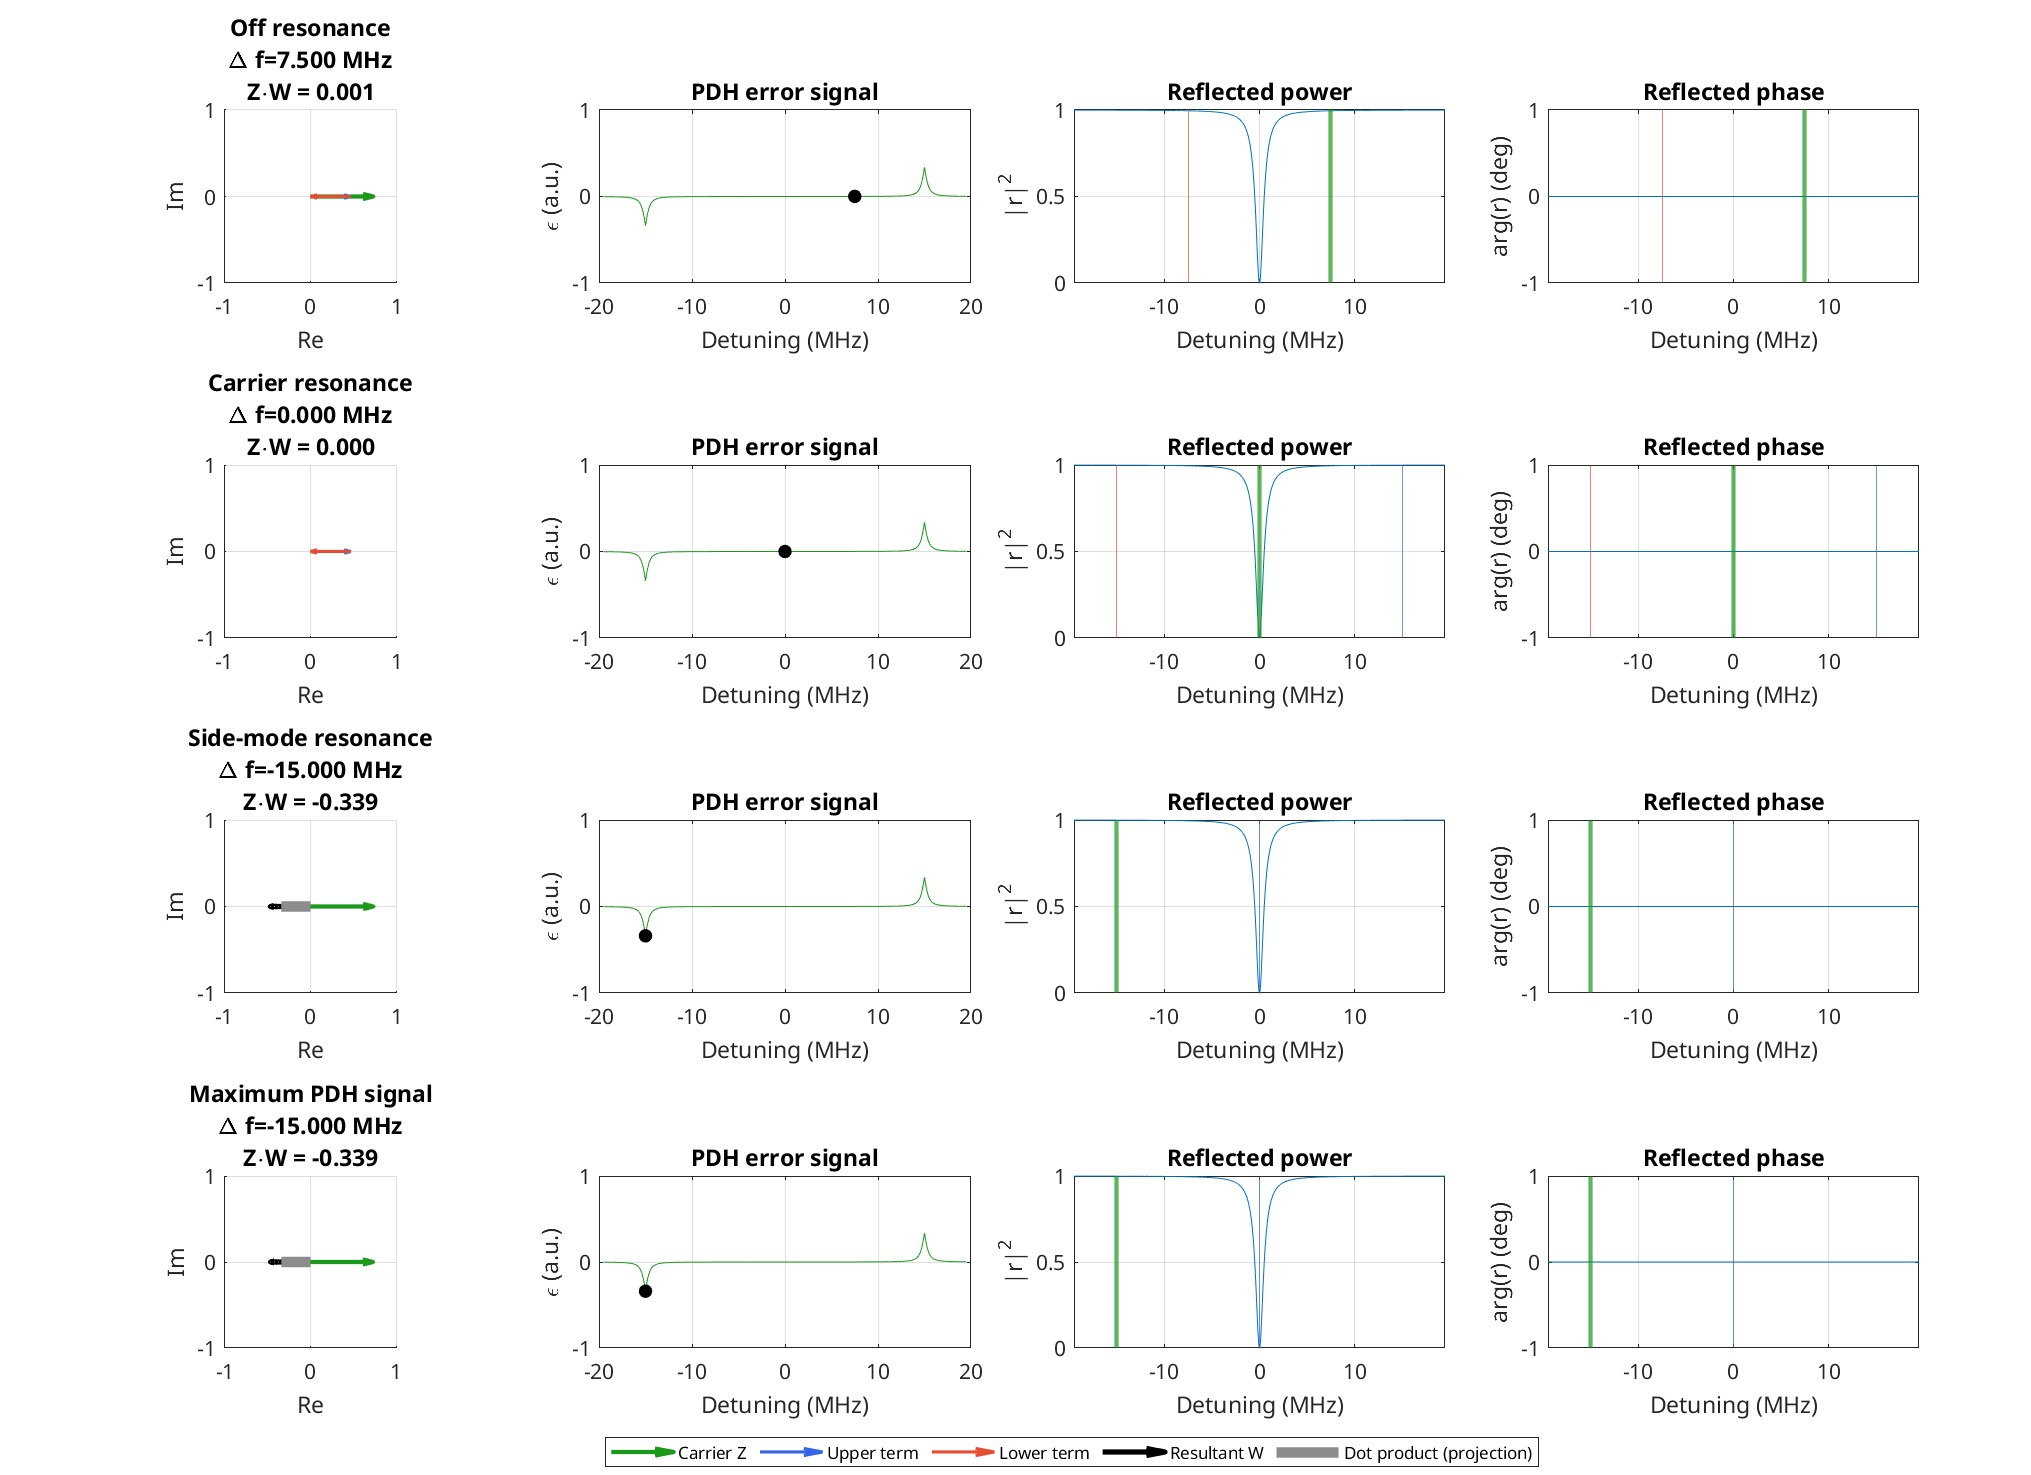
\includegraphics[width=\textwidth]{pic/pdh-resonance-case-walkthrough-absorption.pdf}
\caption{The identical four cases and layout as
Figure~\ref{fig:pdh-resonance-case-walkthrough}, with the cavity's complex
reflection coefficient replaced by its magnitude everywhere, at
$\theta_{\mathrm{demod}}=0$ (Q phase). Reflected phase is flat at
$0^\circ$ in every row: an amplitude-only detector never sees the phase
information Figure~\ref{fig:pdh-resonance-case-walkthrough} relied on.
Cases 3 and 4 coincide exactly.}
\label{fig:pdh-resonance-case-walkthrough-absorption}
\end{figure}

\paragraph{Cases 1 and 2 (absorption-only): still near zero, for a
magnitude reason now.} Off resonance ($\Delta f=f_m/2$), both sidebands sit
at nearly the same background magnitude
($|r(\Delta f+f_m)|\approx|r(\Delta f-f_m)|\approx0.999$), so their
difference --- all that survives at $\theta_{\mathrm{demod}}=0$, since
$\mathcal{E}_{-1}=-\mathcal{E}_1$ turns a sum into a difference here ---
nearly cancels: $\mathcal{E}_{\mathrm{refl,sb}}=0.0009$, giving
$\varepsilon=0.0007$. On carrier resonance, $\mathcal{E}_{\mathrm{refl},0}=0$
exactly, for the identical critical-coupling reason as case 2 above.

\paragraph{Cases 3 and 4 (absorption-only) coincide.} Both land at
$\Delta f=-f_m$, $\varepsilon=-0.339$ --- not forced together, found
independently (case 3 by definition, case 4 by the same numerical search
used in Figure~\ref{fig:pdh-resonance-case-walkthrough}) and agreeing to
within the search grid's own resolution, nine orders of magnitude below
$f_m$. The reason is structural, not coincidental: with phase discarded,
$\mathcal{E}_{\mathrm{refl},0}=\mathcal{E}_0|r(\Delta f)|$ is real and non-negative,
and its magnitude is \emph{minimized}, not extremized, exactly where its
slope is steepest ($\Delta f=0$, critical coupling's own resonance dip)
--- the near-resonance tradeoff that produced case 4's $45^\circ$ point
above (a fast-varying phase carried by a still-substantial magnitude) has
no counterpart here, because there is no phase left to carry it. The only
remaining source of detuning-dependence is
$\mathcal{E}_{\mathrm{refl,sb}}=\mathcal{E}_1\bigl(|r(\Delta f+f_m)|-|r(\Delta f-f_m)|\bigr)$,
an odd, difference-of-two-dips function of $\Delta f$ that is itself
extremized where one dip is entered fully while the other stays at
background --- precisely the side-mode-resonance detuning. Losing phase
does not merely shrink the PDH error signal: it deletes its near-carrier
mechanism outright and replaces it with an on/off sideband-notch effect.
% CHECKED-BY: ReportClaimsDotProductTest.resonanceCaseWalkthroughAmplitudeOnlyCasesCoincide

\bibliographystyle{plain}
\bibliography{references}

\end{document}
